\documentclass{beamer}

\usepackage[T1]{fontenc}
\usepackage[utf8]{inputenc}
\usepackage[french]{babel}
%\usepackage{pslatex}
%\usepackage{colortbl}
%\usepackage{calc}
\usepackage{graphicx}
\usepackage{hyperref}
\usepackage{listings}

\lstset{language=bash,basicstyle=\ttfamily}

\usetheme{Warsaw}

\newcommand{\git}{\texttt{git}}

\definecolor{fondtitre}{rgb}{0.20,0.43,0.09}  % vert fonce
\definecolor{coultitre}{rgb}{0.40,0.04,0.05}  % marron
\definecolor{fondtexte}{rgb}{1,1,1}           % fond blanc
\definecolor{autre1}{RGB}{250,150,5}          % vieux mauve
\definecolor{autre2}{RGB}{235,175,235}        % horrible r
\colorlet{coultexte}{black}

\setbeamercolor{structure}{fg=coultitre, bg=fondtitre!40}
\setbeamercolor{block body}{bg=fondtexte}
\setbeamercolor{normal text}{fg=coultexte,bg=fondtexte}

\setbeamertemplate{navigation symbols}{}

\setbeamertemplate{footline}{
  \hbox{
    \hspace*{-0.06cm}

    \begin{beamercolorbox}[wd=.3\paperwidth,ht=2.25ex,dp=1ex,center]{title in head/foot}
      \usebeamerfont{author in head/foot}\insertshortauthor
      \end{beamercolorbox}

      \begin{beamercolorbox}[wd=.4\paperwidth,ht=2.25ex,dp=1ex,center]{title in head/foot}
      \usebeamerfont{title in head/foot}\insertshorttitle
      \end{beamercolorbox}

      \begin{beamercolorbox}[wd=.1\paperwidth,ht=2.25ex,dp=1ex,center]{date in head/foot}
      \usebeamerfont{date in head/foot}
    \insertframenumber{} / \inserttotalframenumber\hspace*{2ex}
    \end{beamercolorbox}

      \begin{beamercolorbox}[wd=.2\paperwidth,ht=2.25ex,dp=1ex,center]{date in head/foot}
      \usebeamerfont{date in head/foot}\insertdate
      \end{beamercolorbox}}

      \vskip0pt
}

\title[ROSE]{Gestion de versions : \git}
\author{Bertrand, Clément, Laurent, Vaibhav.}
\institute{Télécom ParisTech}
\date{4 mars 2011}

%---------------------------------------

\begin{document}

\begin{frame}
  \titlepage
\end{frame}

%------------------ Plan ---------------
\section*{Plan}
\frame{\frametitle{Plan} \small \tableofcontents}

%------------------ Slides ------------
\section{Introduction}
\subsection*{Présentation des objectifs}
\begin{frame}{Présentation des objectifs}
  \begin{itemize}
  \item Gestionnaire de version ?
  \item Commandes de base
  \item Fonctionnement
  \item Documents additionnels
  \end{itemize}
\end{frame}

\subsection*{Logiciels de gestion de versions}
\begin{frame}{Logiciels de gestion de versions}
  \begin{itemize}
  \item Versionnage d'un projet
  \item Travail en équipe
  \item Résilience aux pannes
  \item Architecture distribuée ou non
  \end{itemize}
\end{frame}

\section{Installer et configurer \git}

\subsection*{Installation}
\begin{frame}{Installation}
  \begin{itemize}
  \item paquets debian/ubuntu : git / éventuellement qgit/git-gui/meld
  \item configuration
  \item initialisation ou clonage
  \end{itemize}
\end{frame}

\subsection*{Configuration}
\begin{frame}[containsverbatim]{Configuration}
  \begin{itemize}
  \item fichier de configuration \lstinline|~/.gitconfig| ou en ligne de commande \lstinline|git config|
  \item
  \end{itemize}
\end{frame}

\section{Les bases de \git}
\subsection*{Statut de fichiers}
\begin{frame}{Statut de fichiers}
  \begin{figure}
    \begin{center}
      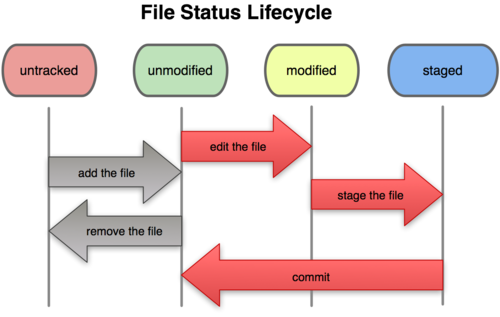
\includegraphics[scale=0.7]{img/Status_lifecycle.png}
    \end{center}
    \caption{progit.org}
  \end{figure}
\end{frame}

\subsection*{Commandes de Base}
\begin{frame}[containsverbatim]{Commandes de Base}
  \begin{itemize}
  \item \lstinline|git clone| - clone un dépôt distant \lstinline|git clone [url]| 
\begin{lstlisting}
$ git clone git://github.com/schacon/grit.git
\end{lstlisting}
  \item \lstinline|git status| - Afficher l'état de l'arbre de travail
\begin{lstlisting}
$ git status
# On branch master
nothing to commit (working directory clean)
\end{lstlisting}
\end{itemize}
\end{frame}

\begin{frame}[containsverbatim]{Commandes de Base...}
  \begin{itemize}

\item \lstinline|git log <filename>| - Afficher commettre journaux. avec -p, afficher patch aussi 
\begin{lstlisting}
$ git log git.tex 
commit 8fdb1efff1b859109718ec6c1015ee97a168dc93 
Author: Bertrand Chazot <chazot@enst.fr> 
Date:   Tue Mar 1 17:21:17 2011 +0100 
minor fixs

commit cbd5a7ad5603ef3e33cfc00b9ea119519fcaf1fe 
Author: Clement Moussu <moussu@telecom-paristech.fr>
Date:   Mon Feb 28 22:45:03 2011 +0100

Fixups.
\end{lstlisting}
\end{itemize}
\end{frame}

\begin{frame}[containsverbatim]{Commandes de Base...}
  \begin{itemize}
\item \lstinline|git diff| - Afficher les modifications entre les engage, l'engagement et de travail des arbres, etc
\begin{lstlisting}
$ git diff git.tex
diff --git a/git.tex b/git.tex
index bc5d0e8..d0d5409 100644
--- a/git.tex
+++ b/git.tex
@@ -123,6 +123,16 @@
end{figure}
end{frame}
\end{lstlisting}

\end{itemize}
\end{frame}
\begin{frame}[containsverbatim]{Commandes de Base...}
  \begin{itemize}
\item \lstinline|git add| - ajoute de nouveaux objets "blobs" dans la base des objets pour chaque fichier modifié depuis le dernier commit.
Les objets précédents restent inchangés.
\begin{lstlisting}
$ git add git.tex
\end{lstlisting}

\item \lstinline|git add -u| - Mises à jour des changements dans les fichiers déjà "staged"

  \end{itemize}
\end{frame}

\begin{frame}[containsverbatim]{Commandes de Base...}
  \begin{itemize}
\item \lstinline|git diff --cached|- Afficher les modifications sur la "staged" zone.
\begin{lstlisting}
$ git diff --cached git.tex
\end{lstlisting}

\item \lstinline|git reset HEAD <filename>| 
\begin{lstlisting}
$ git reset HEAD git.tex
Unstaged changes after reset:
M       git.tex
\end{lstlisting}

\item \lstinline|git rm|- Supprimer les fichiers de l'arbre de travail et de l'indice 
\begin{lstlisting}
$ git rm git.tex
\end{lstlisting}
\item \lstinline|git rm --cached|
    
  \end{itemize}
\end{frame}
\begin{frame}[containsverbatim]{Commandes de Base...}
  \begin{itemize}
\item \lstinline|git commit|-Enregistrez les changements au dépôt "local"
\begin{lstlisting}
$ git commit
$ git commit git.tex
\end{lstlisting}

\item \lstinline|git commit -a| 
\begin{lstlisting}
$ git commit -a
\end{lstlisting}
  
  \end{itemize}
\end{frame}

%------------------------------------------------------------
% Clément & Bertrand

\section{Gestion de branches}
\subsection*{Gestion locale}
\begin{frame}{Gestion locale 1/2}
  \begin{figure}
    \begin{center}
      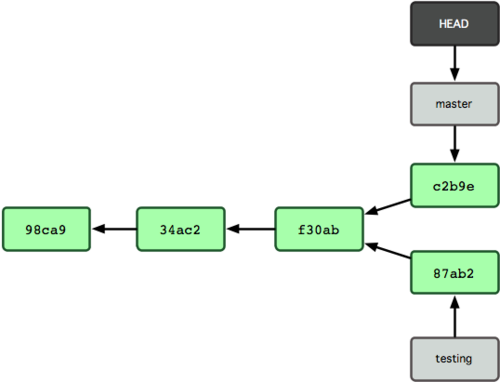
\includegraphics[scale=0.7]{img/Branch1.png}
    \end{center}
    \caption{progit.org}
  \end{figure}
\end{frame}

\begin{frame}[containsverbatim]{Gestion locale 2/2}
  \begin{itemize}
  \item Lister les branches : \lstinline|git branch|
  \item Lister les branches mergées avec la branche courante : \lstinline|git branch|
  \item Lister les branches non mergées avec la branche courante : \lstinline|git branch|
  \item Lister les branches : \lstinline|git branch|
  \item Créer une branche : \lstinline|git branch <name>|
  \item Supprimer une branche : \lstinline|git branch -d <name>|
  \item Déplacer HEAD vers branch : \lstinline|git checkout <branch>|
  \item Création et déplacer HEAD : \lstinline|git checkout -b <branch>|
  \item Log, dernier commit de chaque branche : \lstinline|git branch -v|
  \end{itemize}
\end{frame}

\subsection*{Communication avec le serveur}
\begin{frame}{Communication avec le serveur 1/2}
  \begin{itemize}
  \item Fetch
  \item Push
  \item Pull
  \item Tracking : push -u / checkout --track / git checkout -b
  \end{itemize}
\end{frame}

\begin{frame}{Communication avec le serveur 2/2}
  \begin{figure}
    \begin{center}
      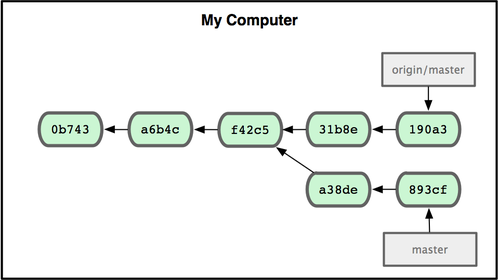
\includegraphics[scale=0.7]{img/RemoteBranch.png}
    \end{center}
    \caption{progit.org}
  \end{figure}
\end{frame}

\subsection*{Merger}
\begin{frame}{Merger 1/2}
  \begin{itemize}
  \item Merge
  \end{itemize}
\end{frame}

\begin{frame}{Merger 2/2}
  \begin{figure}
    \begin{center}
      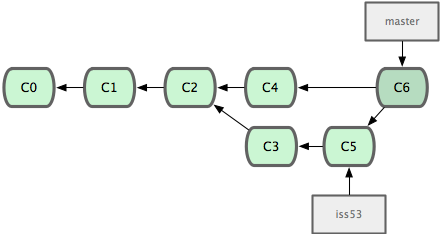
\includegraphics[scale=0.7]{img/Merge.png}
    \end{center}
    \caption{progit.org}
  \end{figure}
\end{frame}

\subsection*{Rebase}
\begin{frame}{Rebase 1/2}
  \begin{itemize}
  \item r
  \end{itemize}
\end{frame}

\begin{frame}{Rebase 2/2}
  \begin{figure}
    \begin{center}
    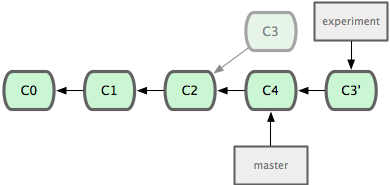
\includegraphics[scale=0.7]{img/Rebase.png}
    \end{center}
    \caption{progit.org}
  \end{figure}
\end{frame}

\begin{frame}{}
  \begin{columns}
    \begin{column}{0.60\textwidth}
      \begin{itemize}
      \item \lstinline|git clone user@host:repo.git|
      \end{itemize}
    \end{column}
    \begin{column}{0.40\textwidth}
      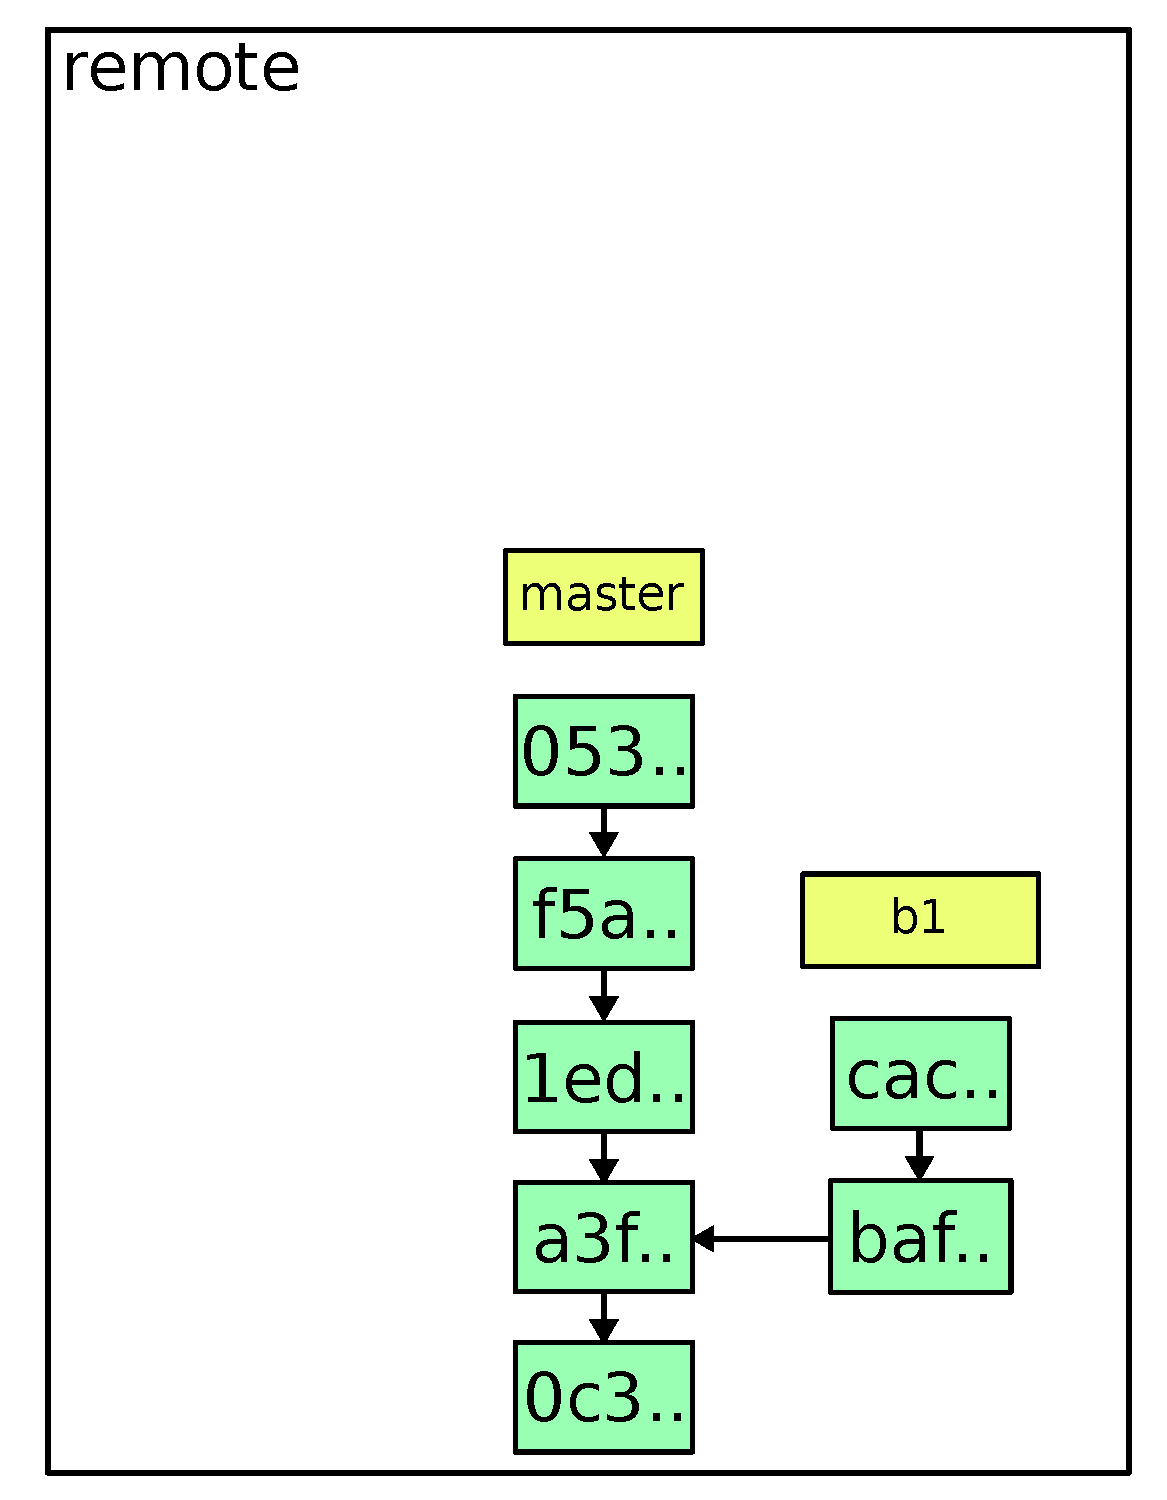
\includegraphics[width=\textwidth]{img/1.pdf}
    \end{column}
  \end{columns}
\end{frame}

\begin{frame}{}
  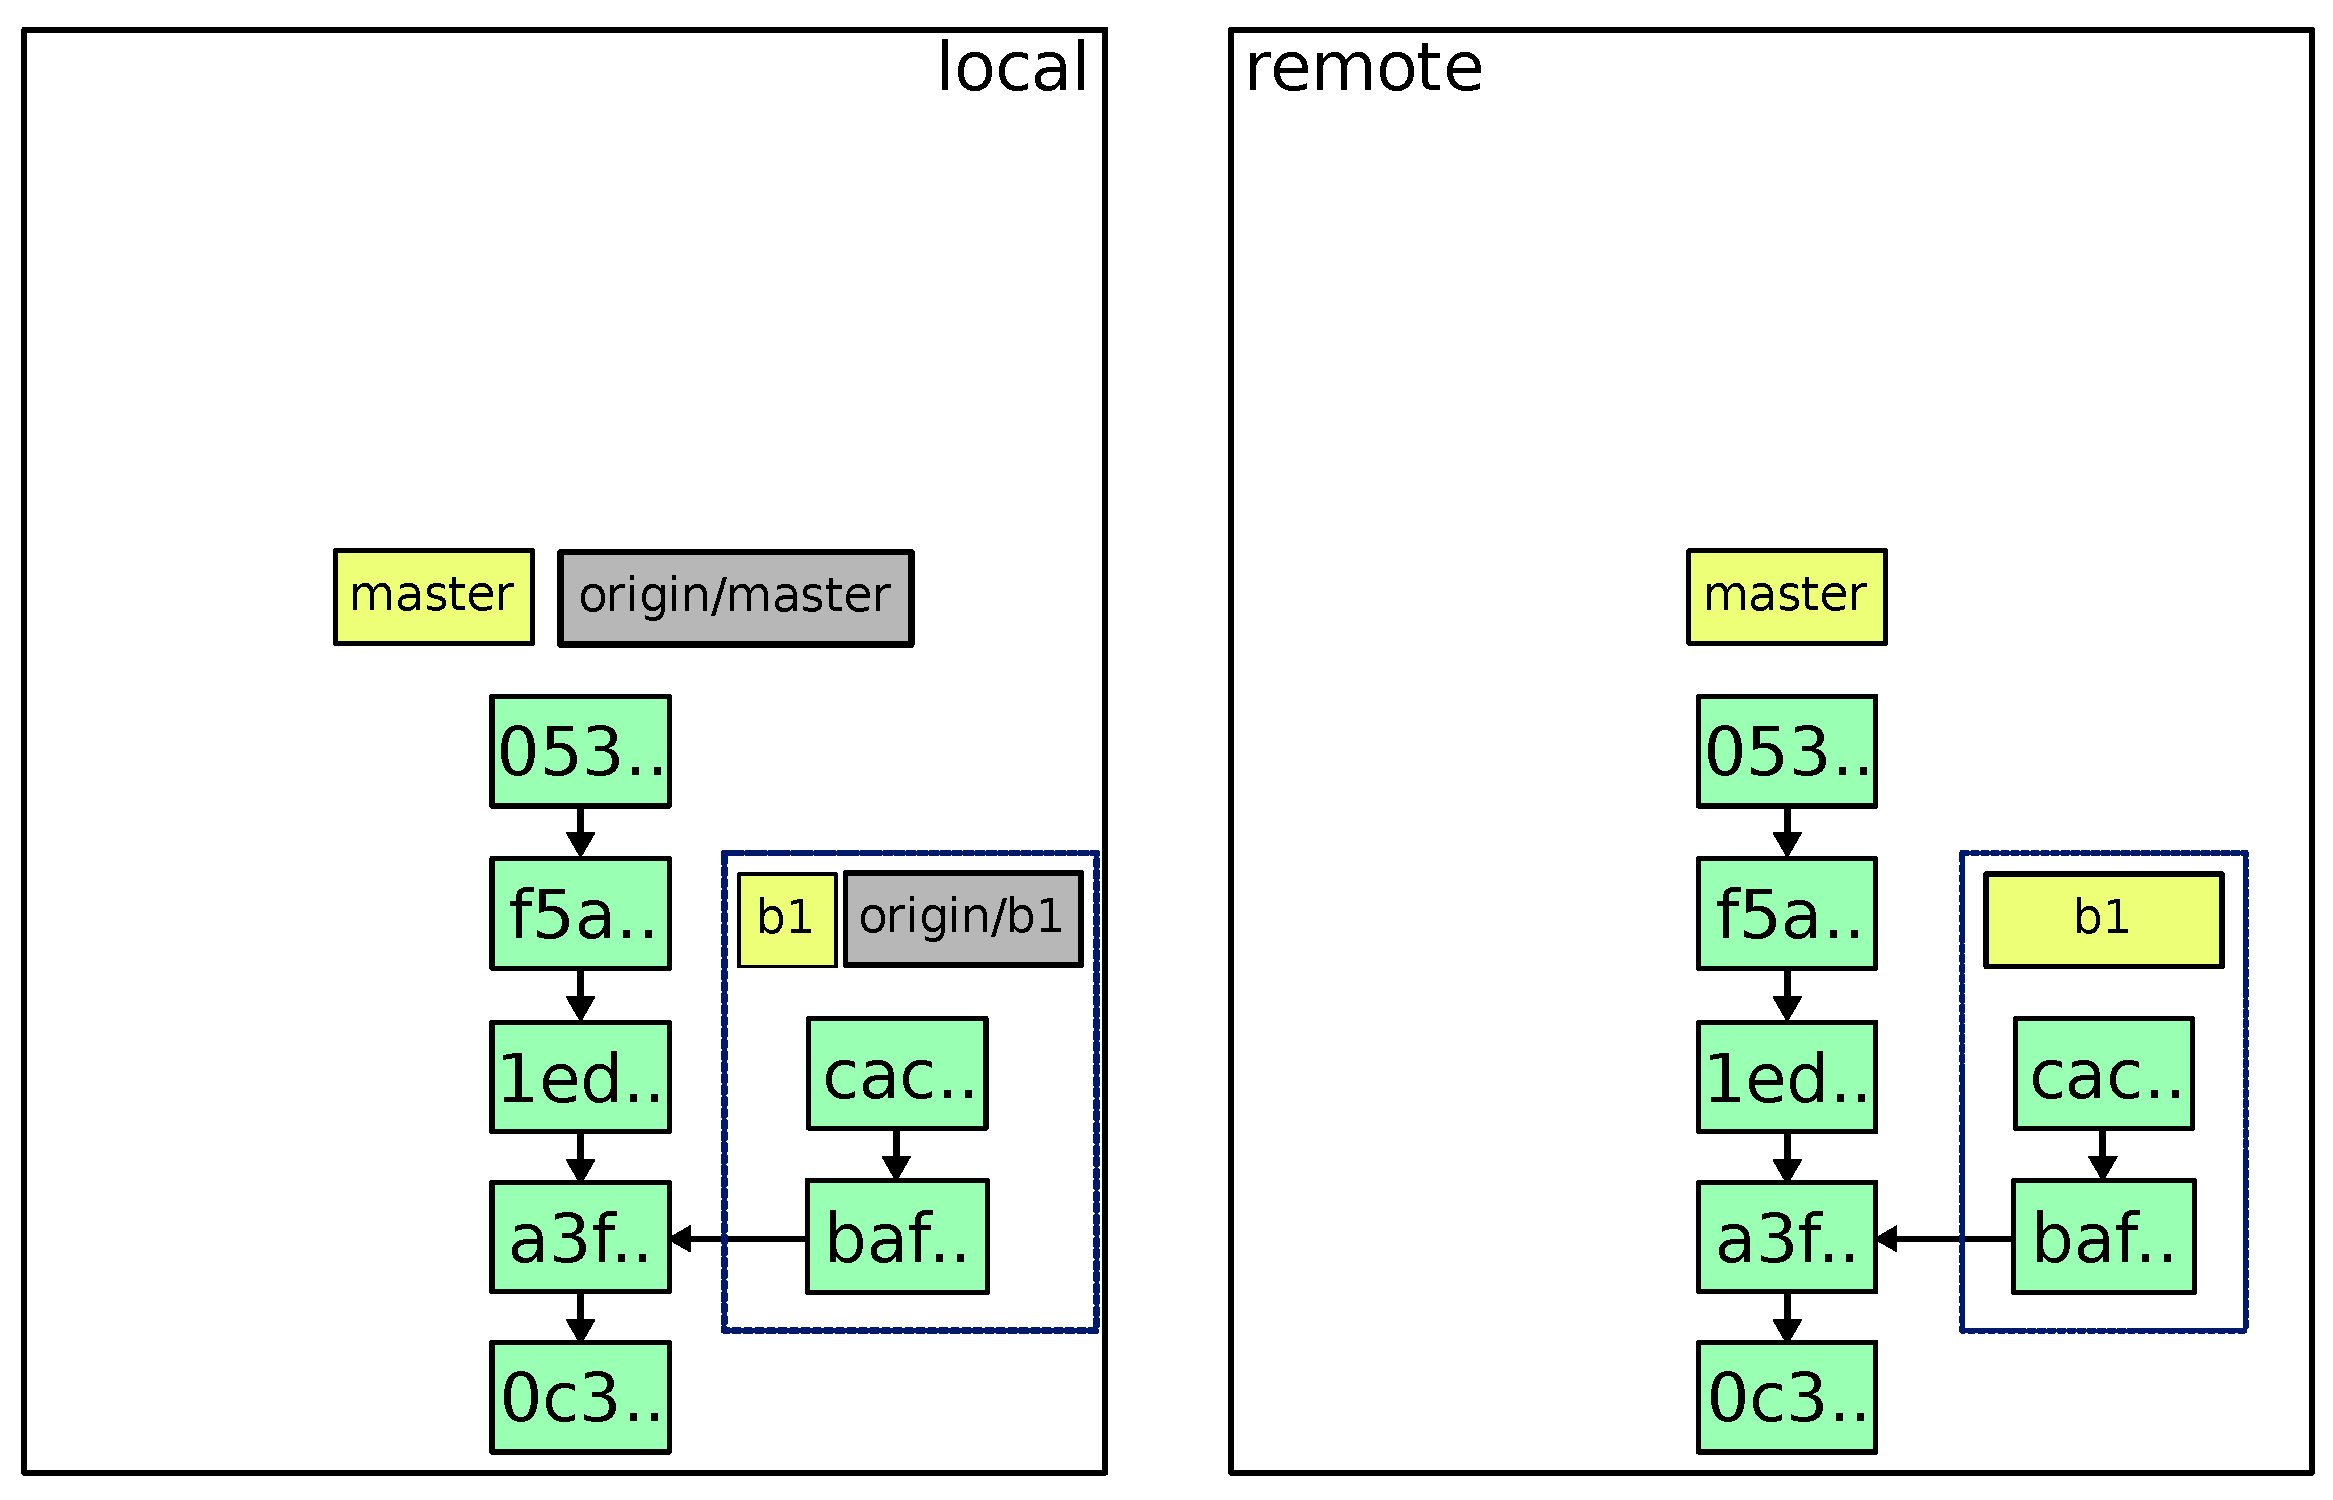
\includegraphics[width=\textwidth]{img/2.pdf}
\end{frame}

\begin{frame}{}
  \begin{itemize}
  \item \lstinline|git checkout master|
  \item \lstinline|git branch b2|
  \item \lstinline|git checkout b2|
  \end{itemize}
\end{frame}

\begin{frame}{}
  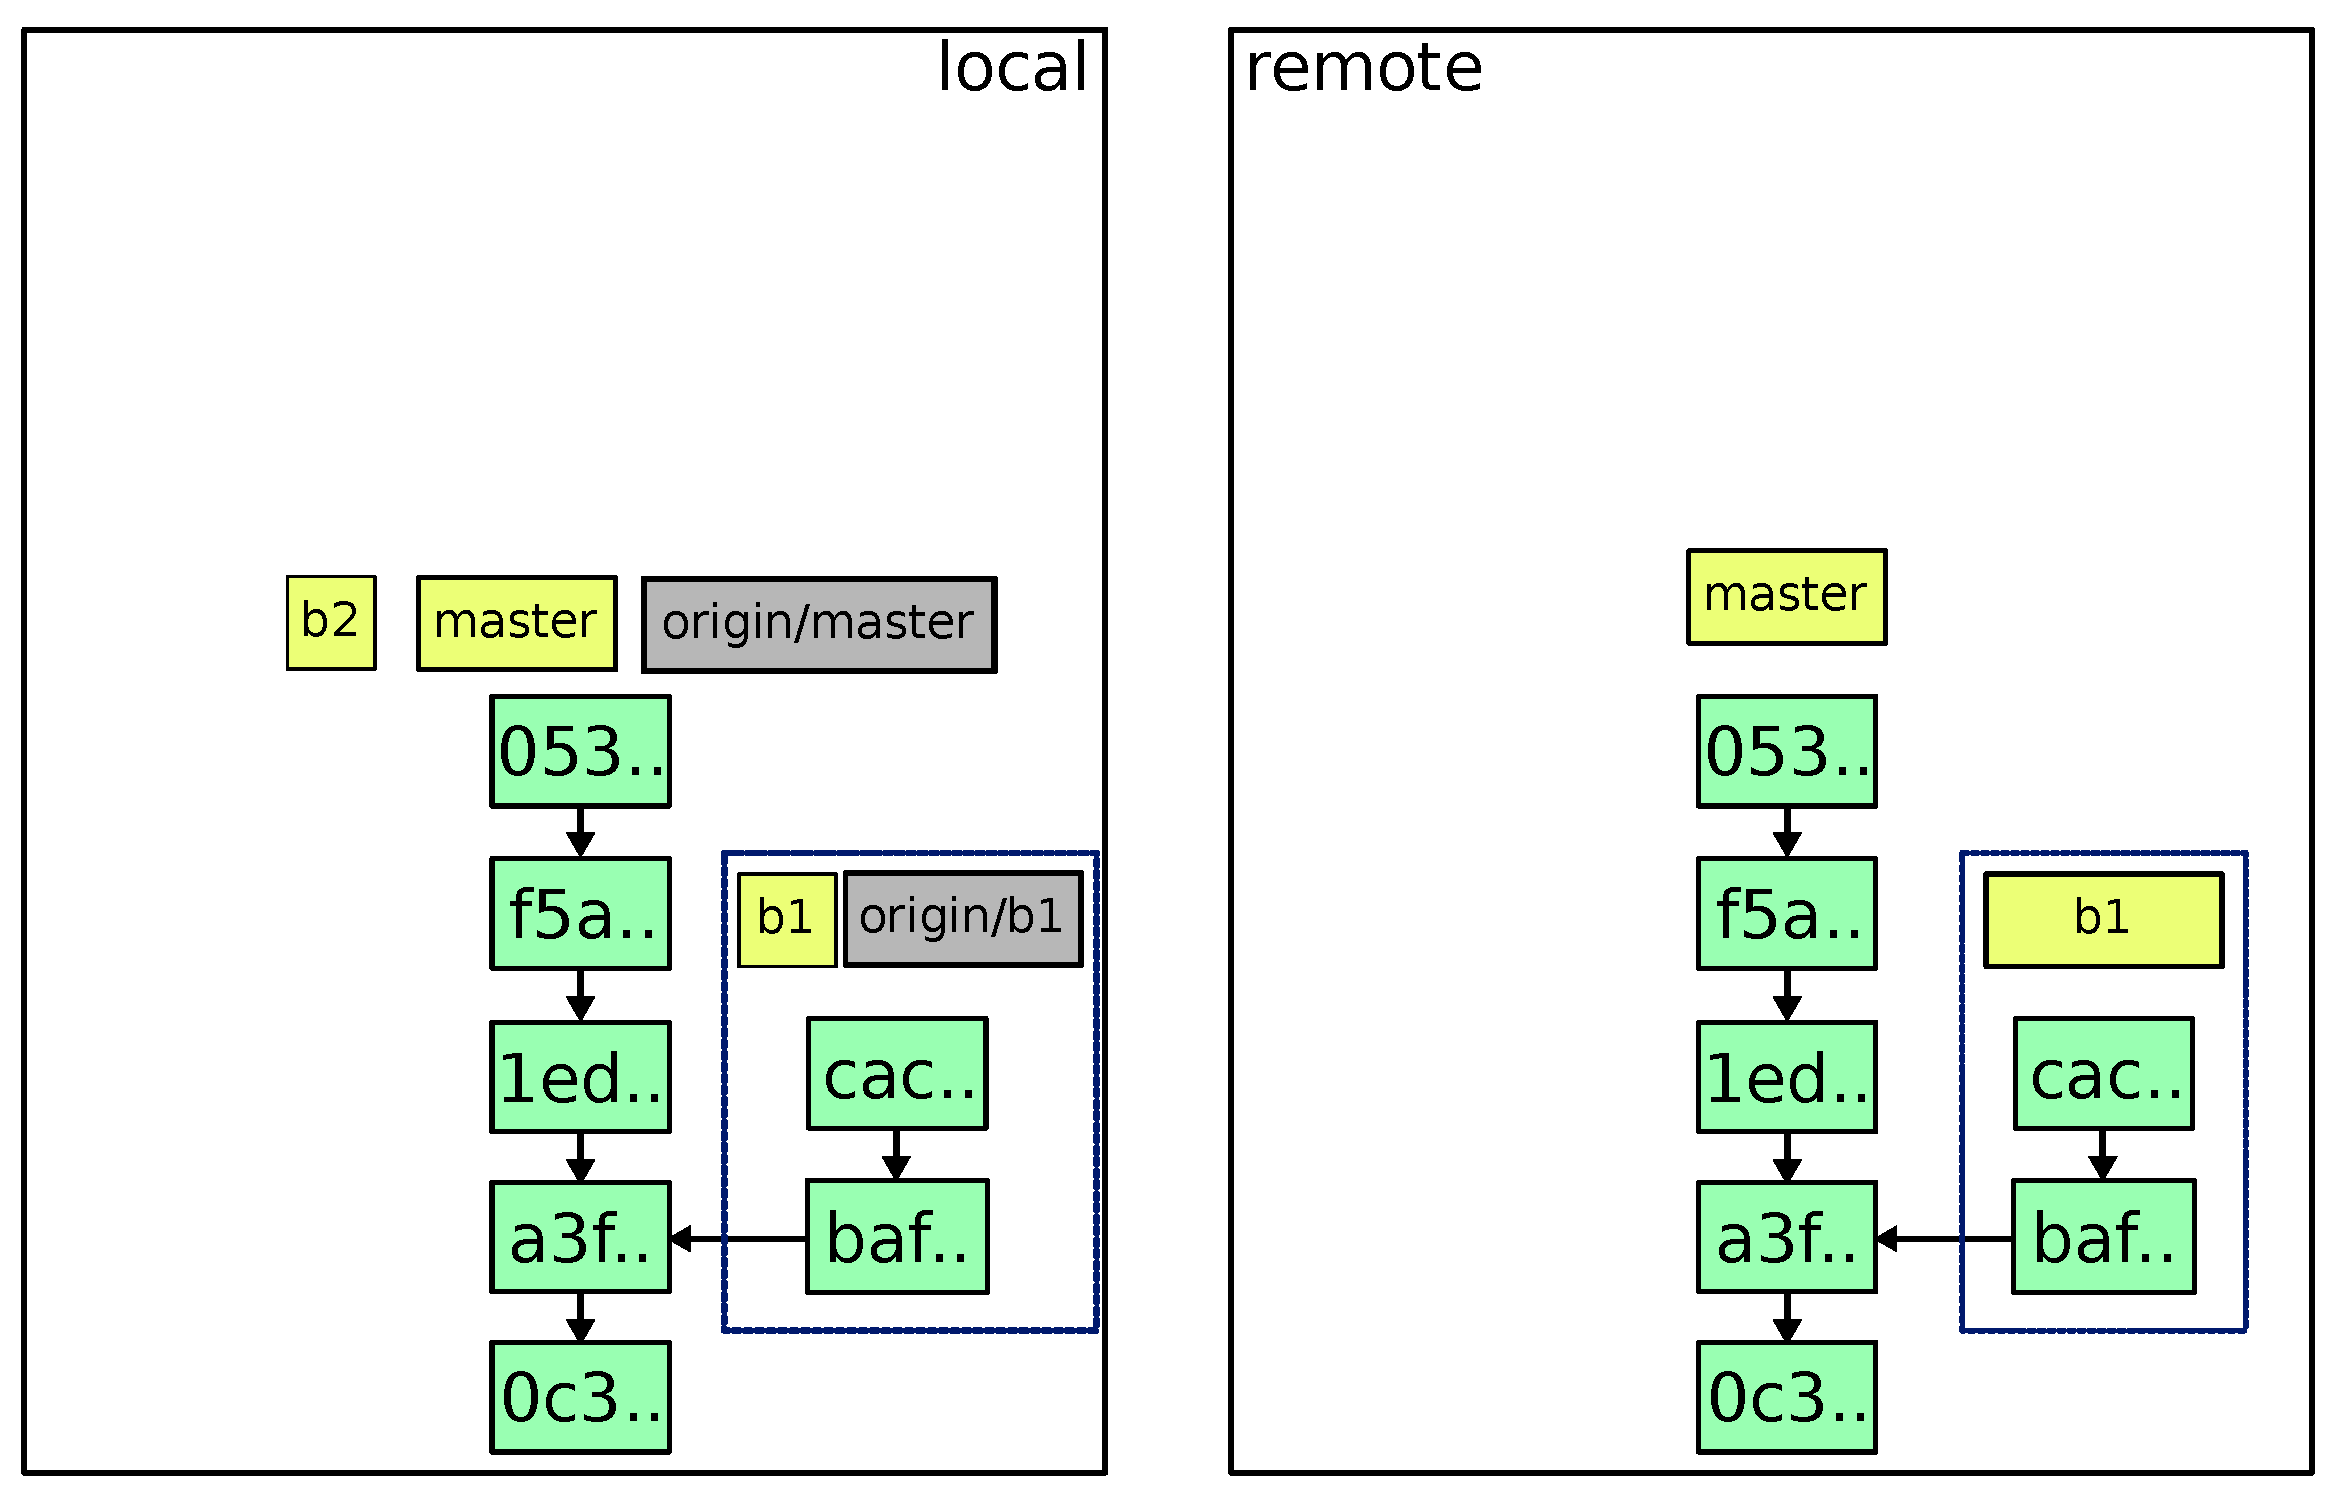
\includegraphics[width=\textwidth]{img/3.pdf}
\end{frame}

\begin{frame}{}
  \begin{itemize}
  \item do some changes
  \item \lstinline|git add <files>|
  \item \lstinline|git commit|
  \end{itemize}
\end{frame}

\begin{frame}{}
  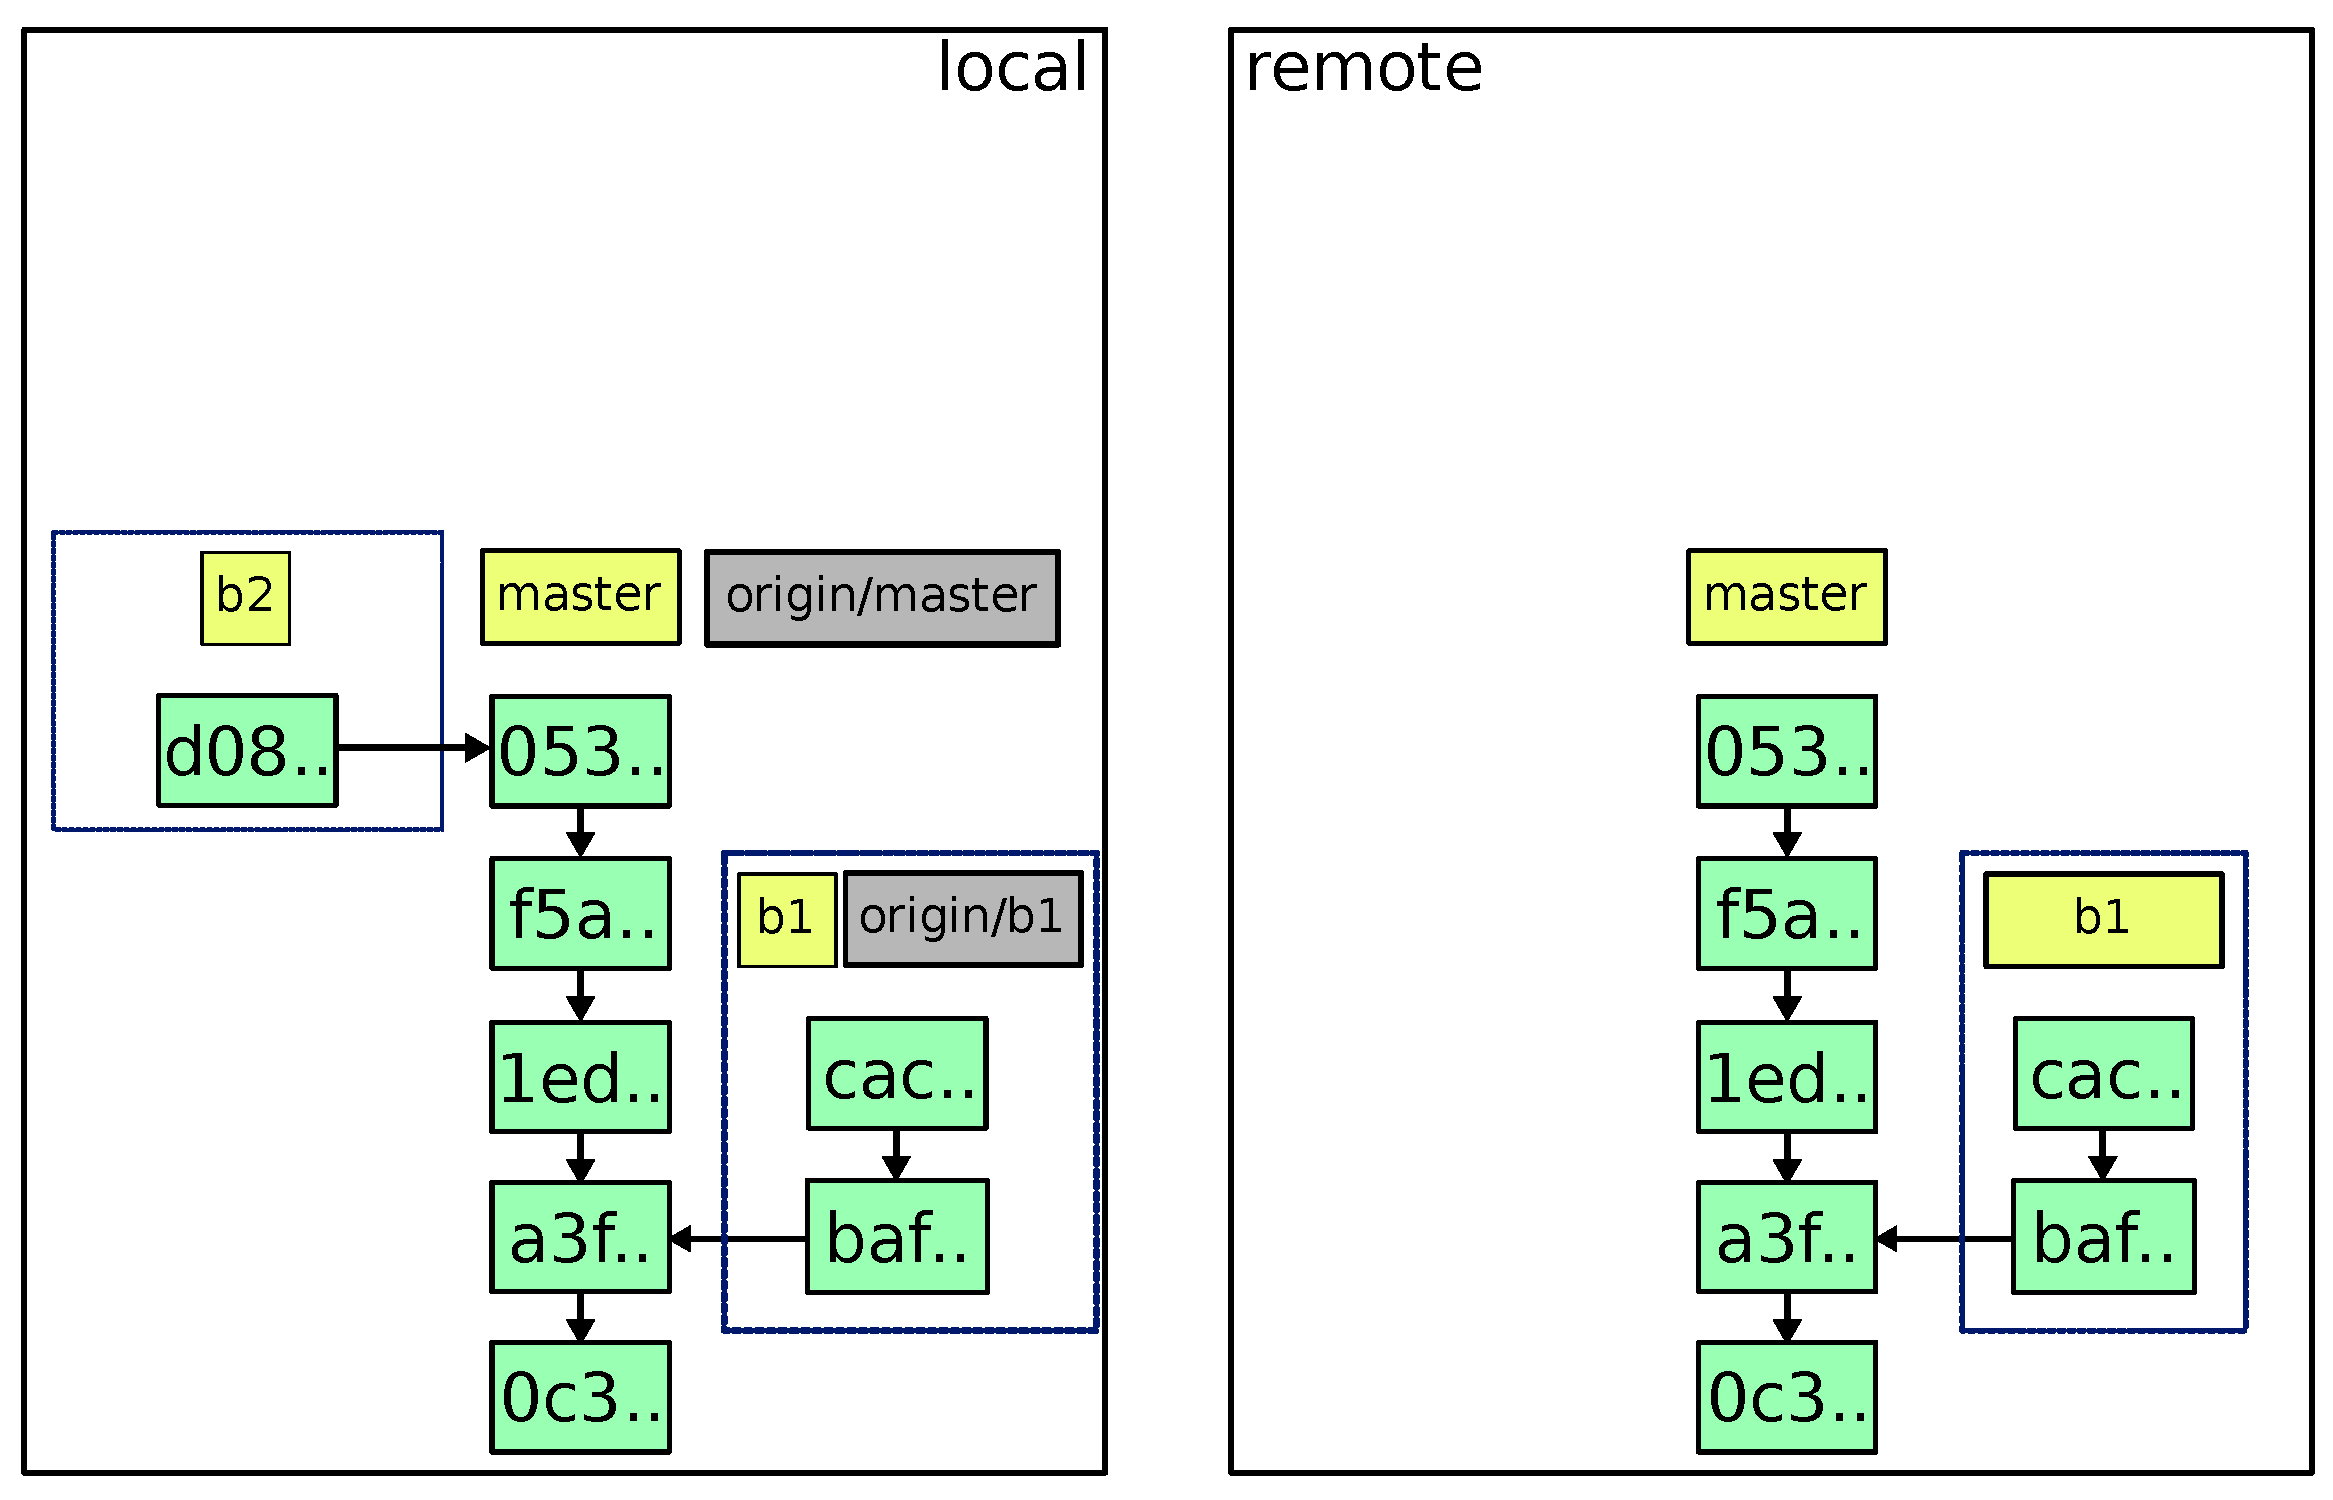
\includegraphics[width=\textwidth]{img/3-bis.pdf}
\end{frame}

\begin{frame}{}
  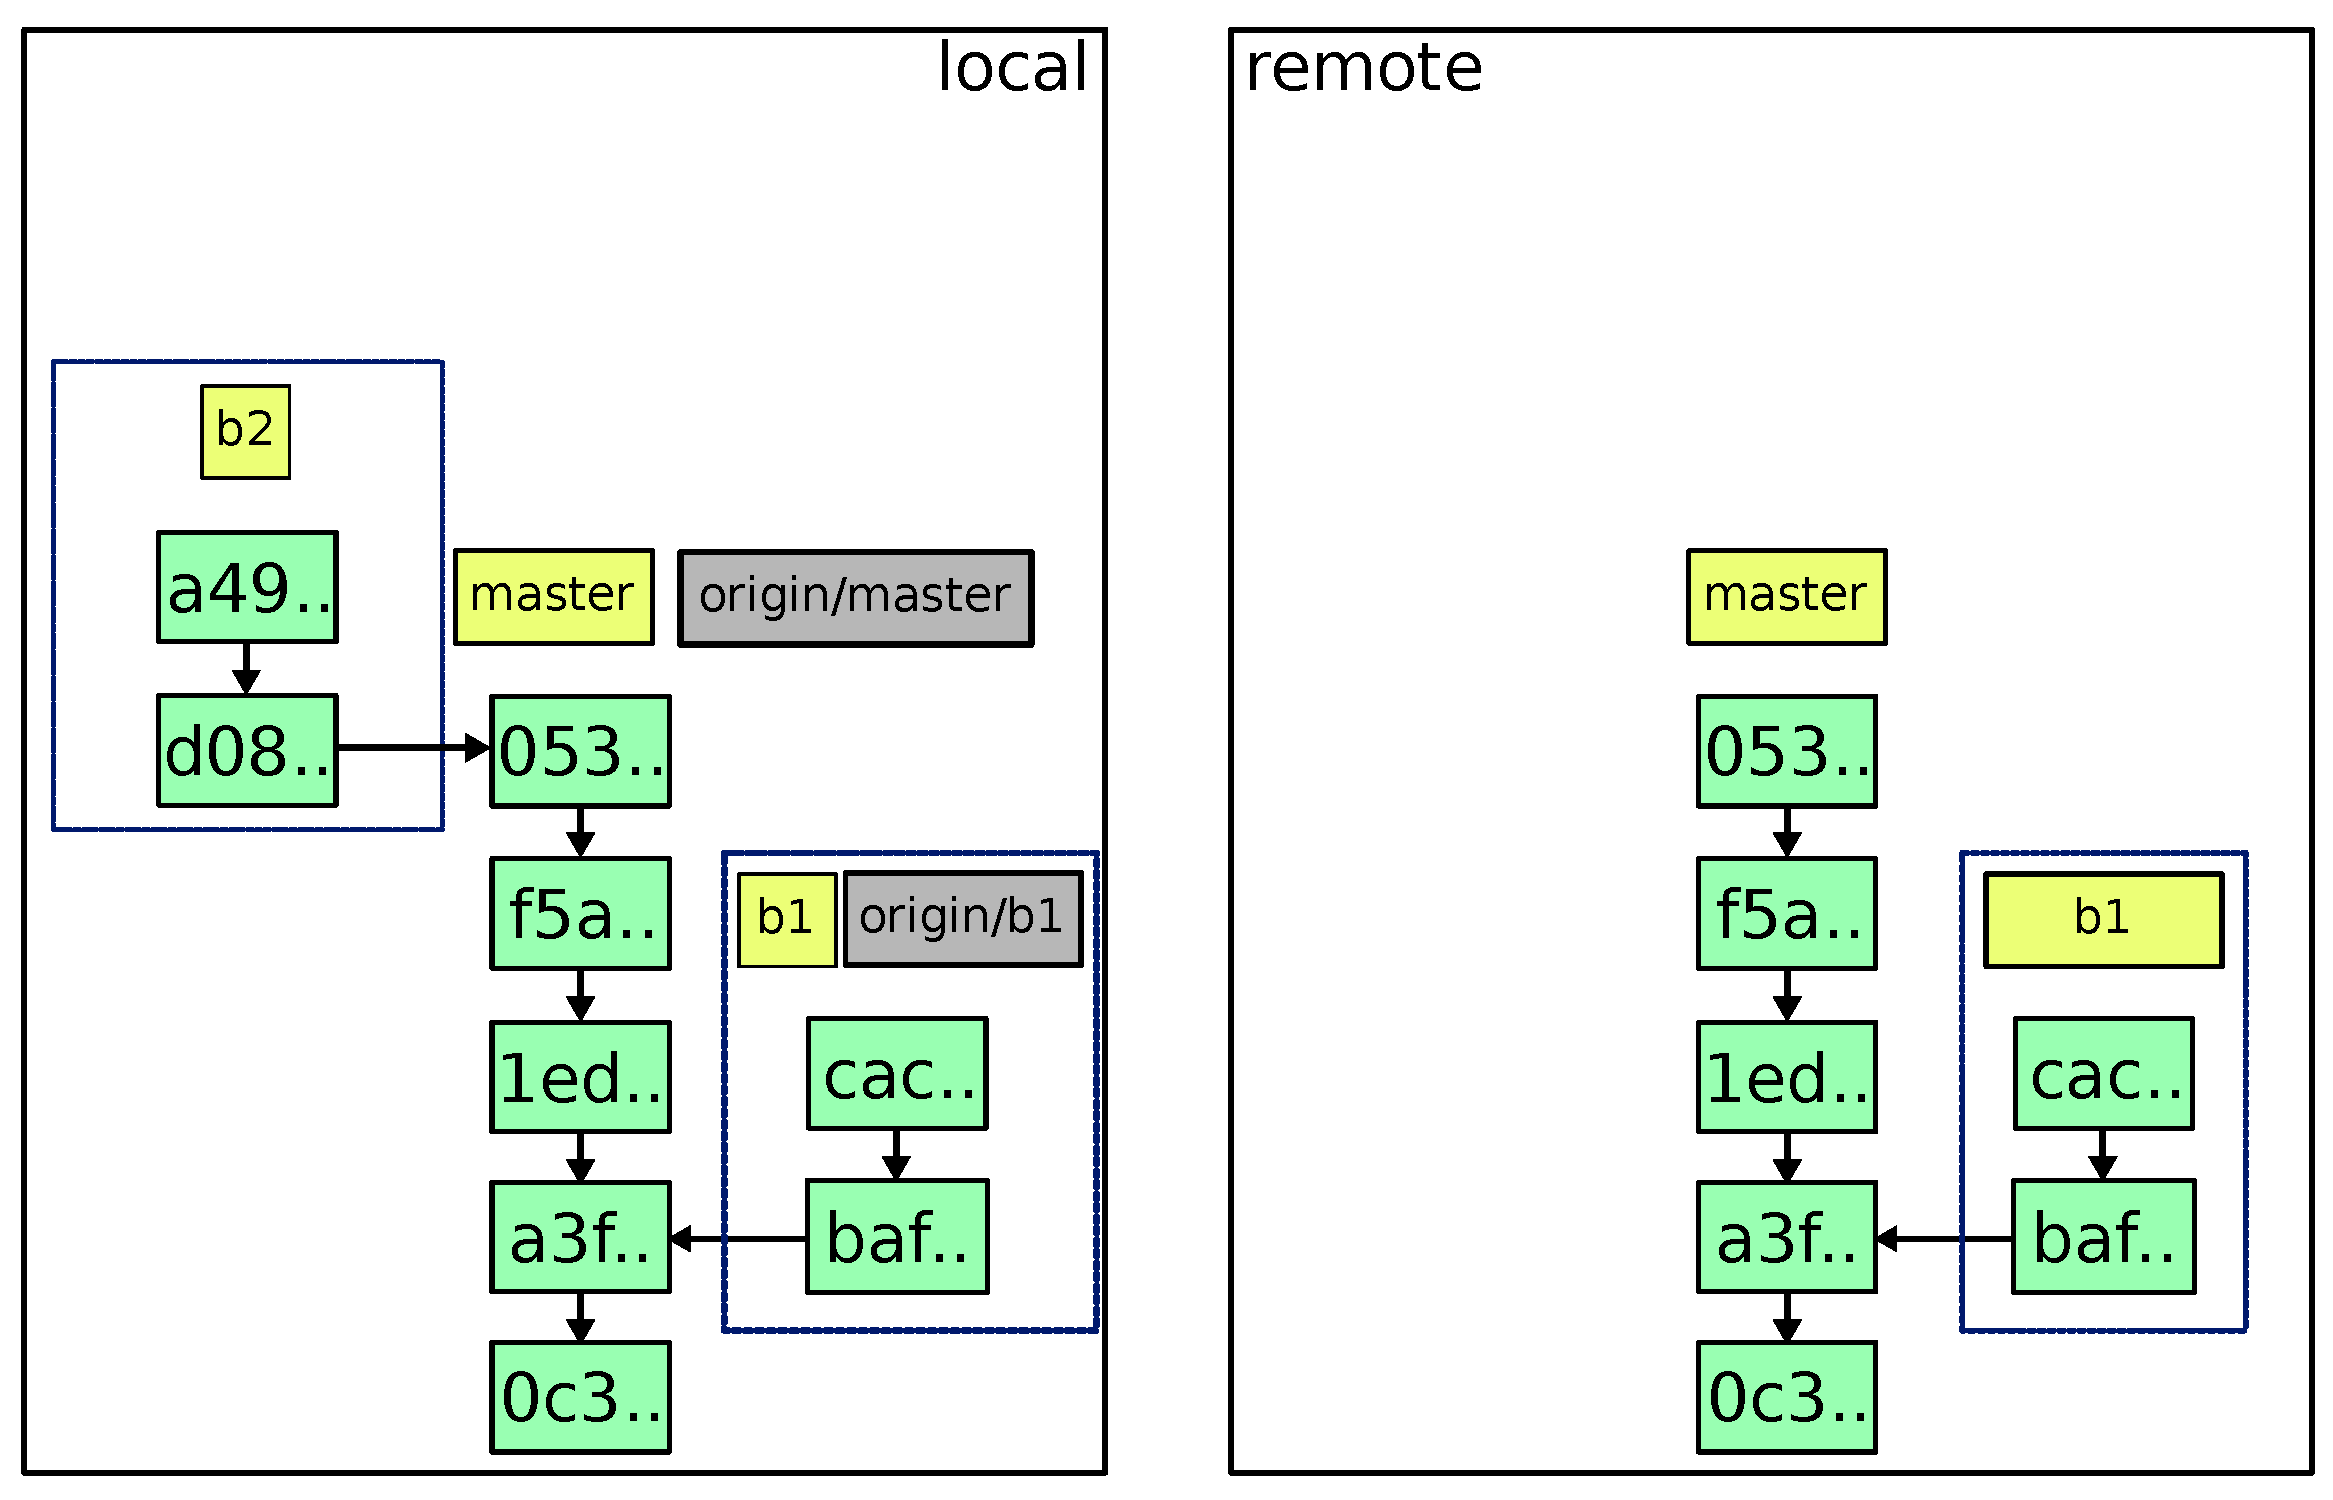
\includegraphics[width=\textwidth]{img/3-ter.pdf}
\end{frame}

\begin{frame}{}
  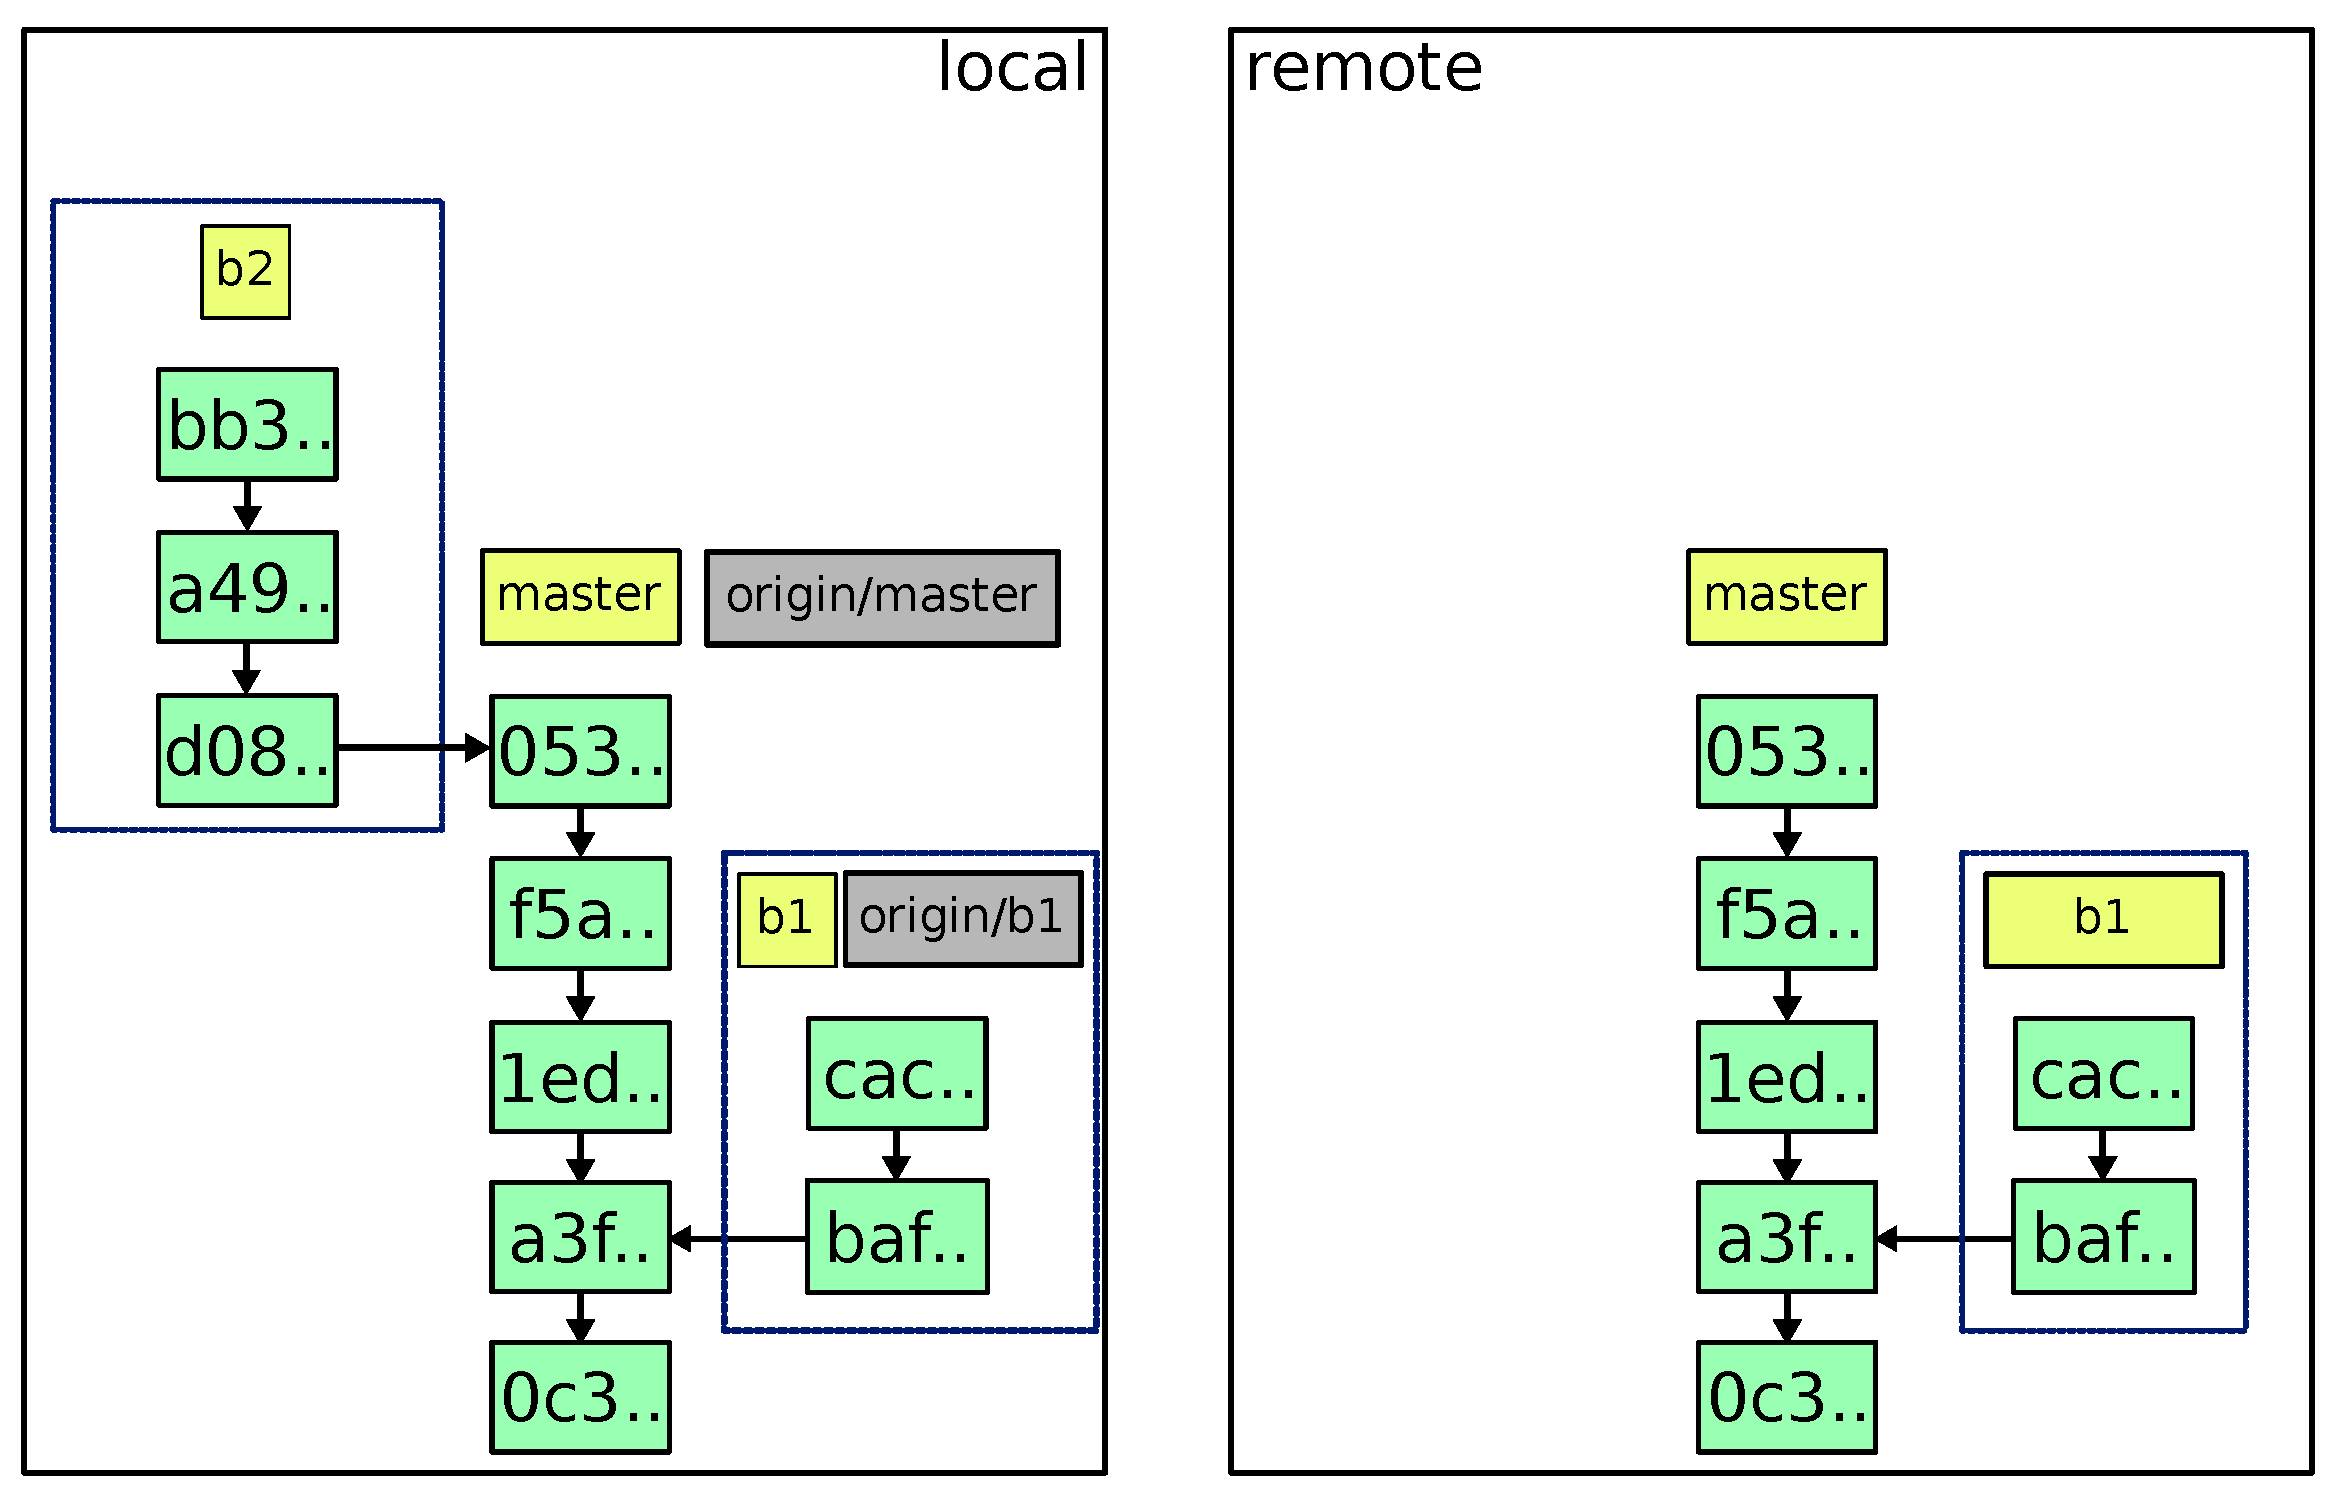
\includegraphics[width=\textwidth]{img/3-quad.pdf}
\end{frame}

\begin{frame}{}
  \begin{itemize}
  \item \lstinline|git push origin b2|
  \end{itemize}
\end{frame}

\begin{frame}{}
  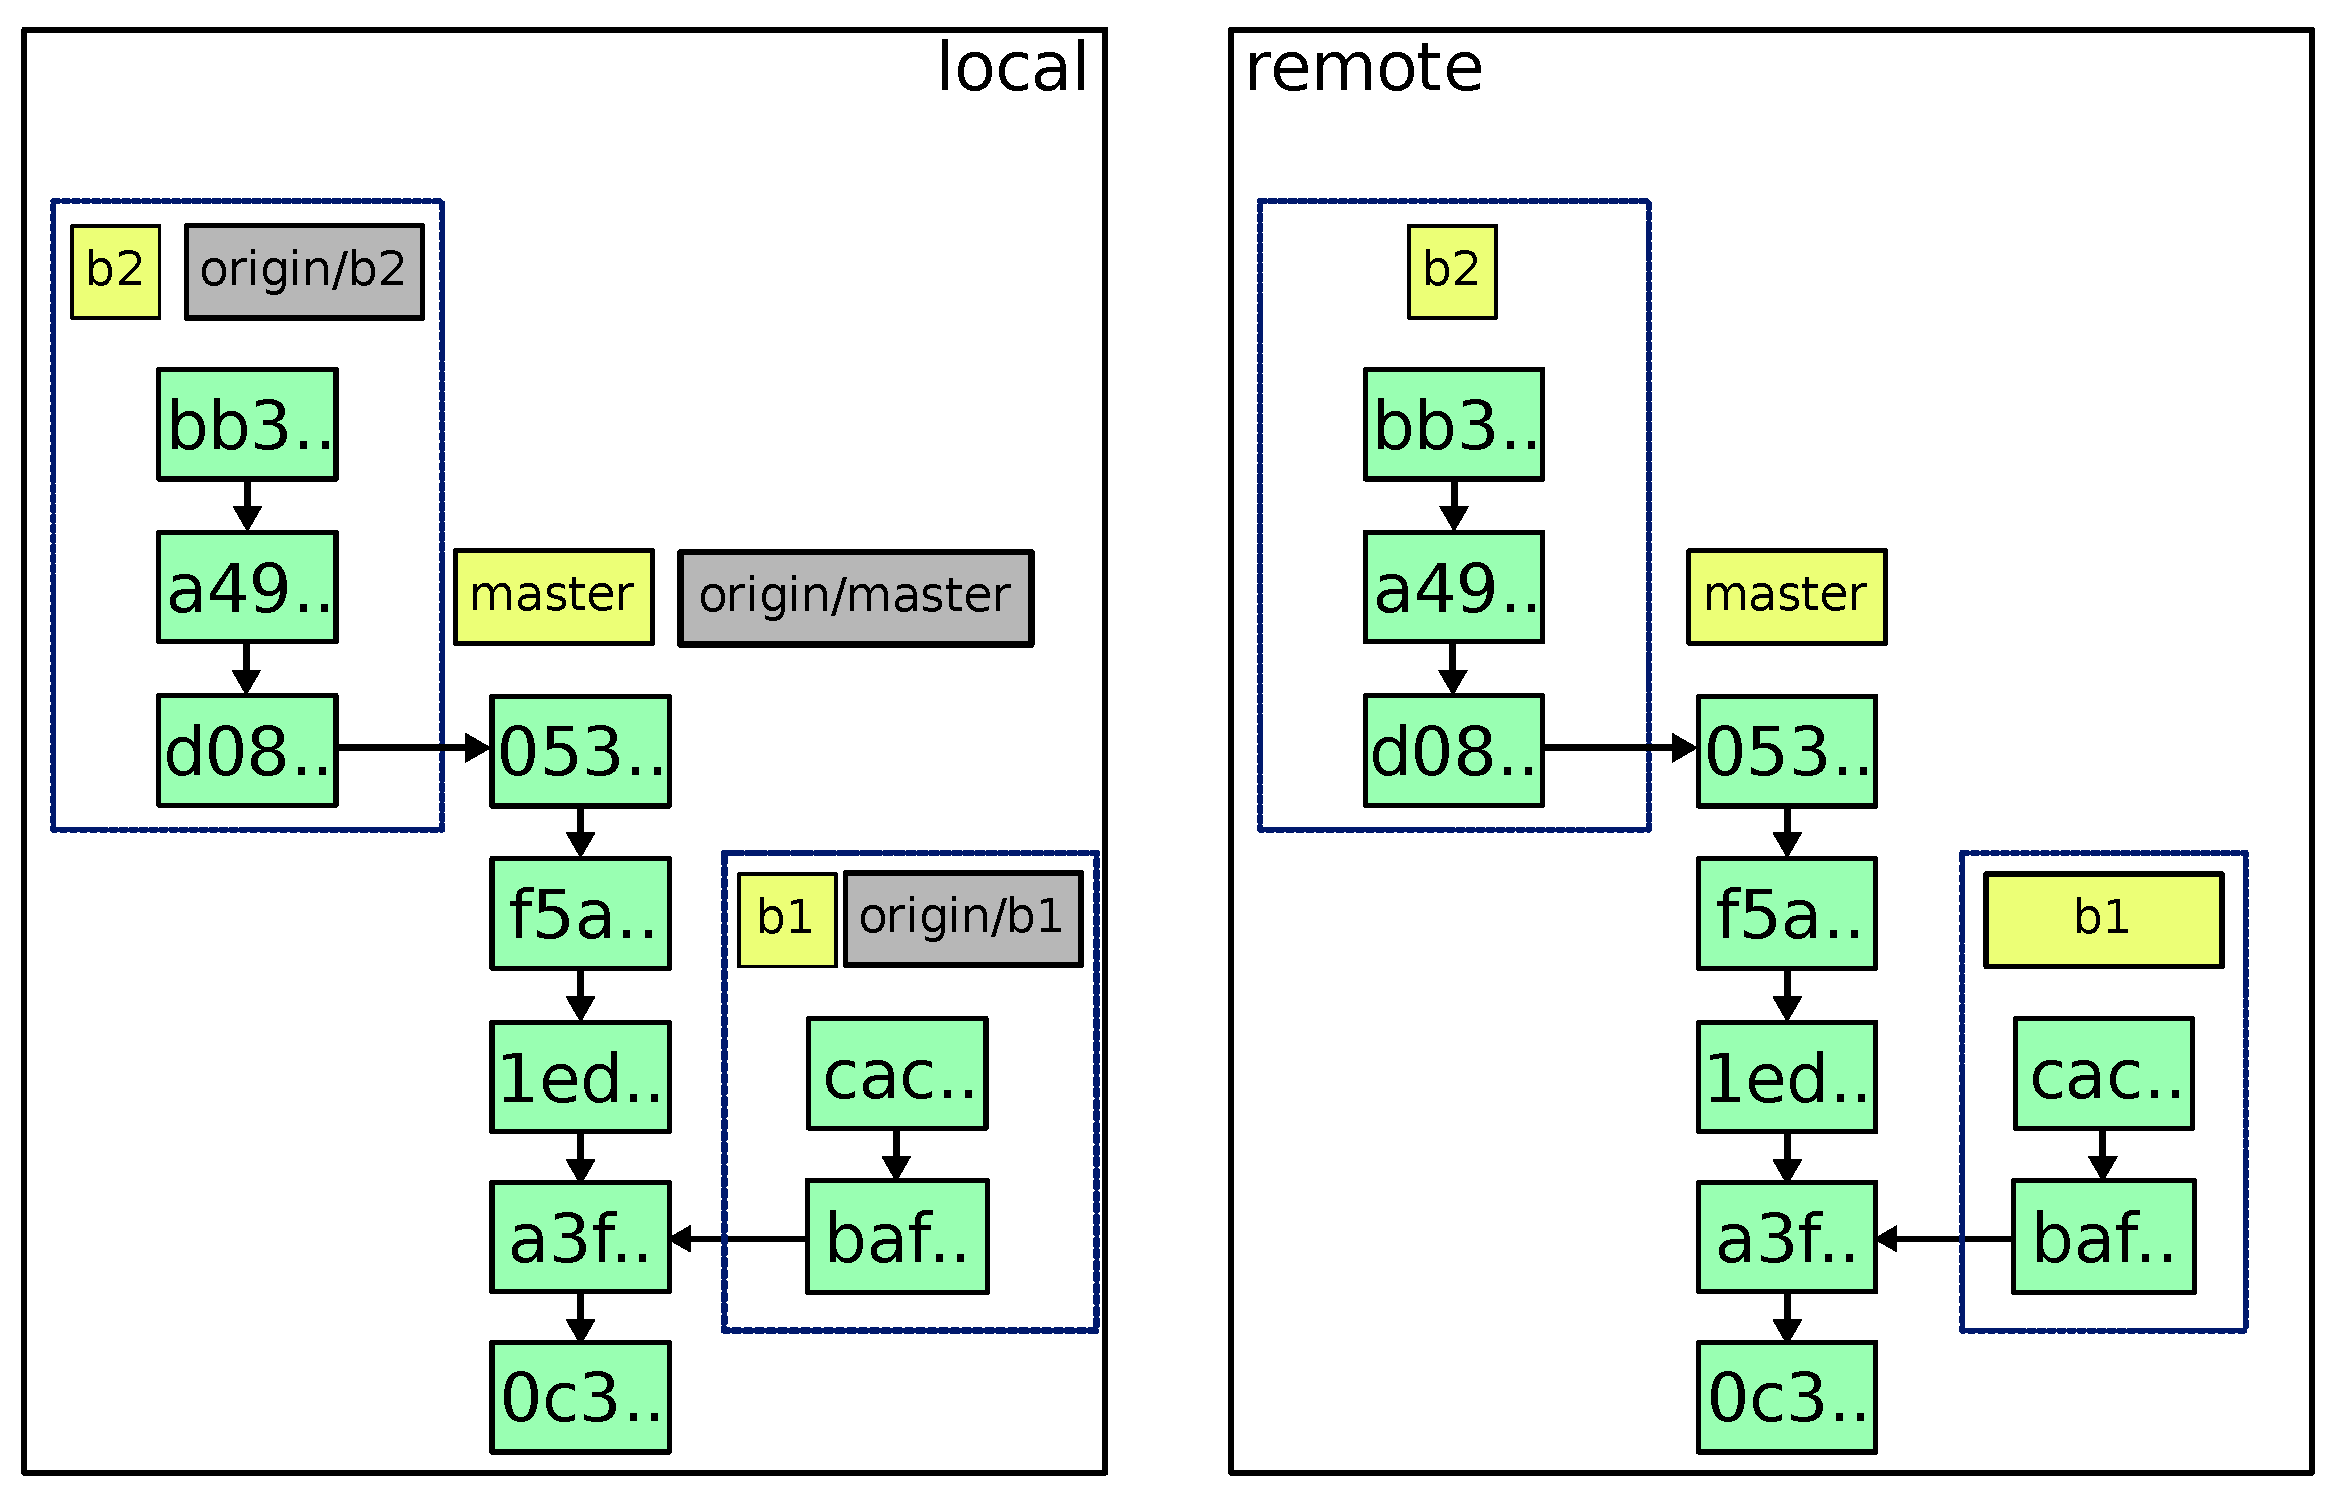
\includegraphics[width=\textwidth]{img/4.pdf}
\end{frame}

\begin{frame}{}
  \begin{itemize}
  \item \lstinline|git rebase master b1|
  \end{itemize}
\end{frame}

\begin{frame}{}
  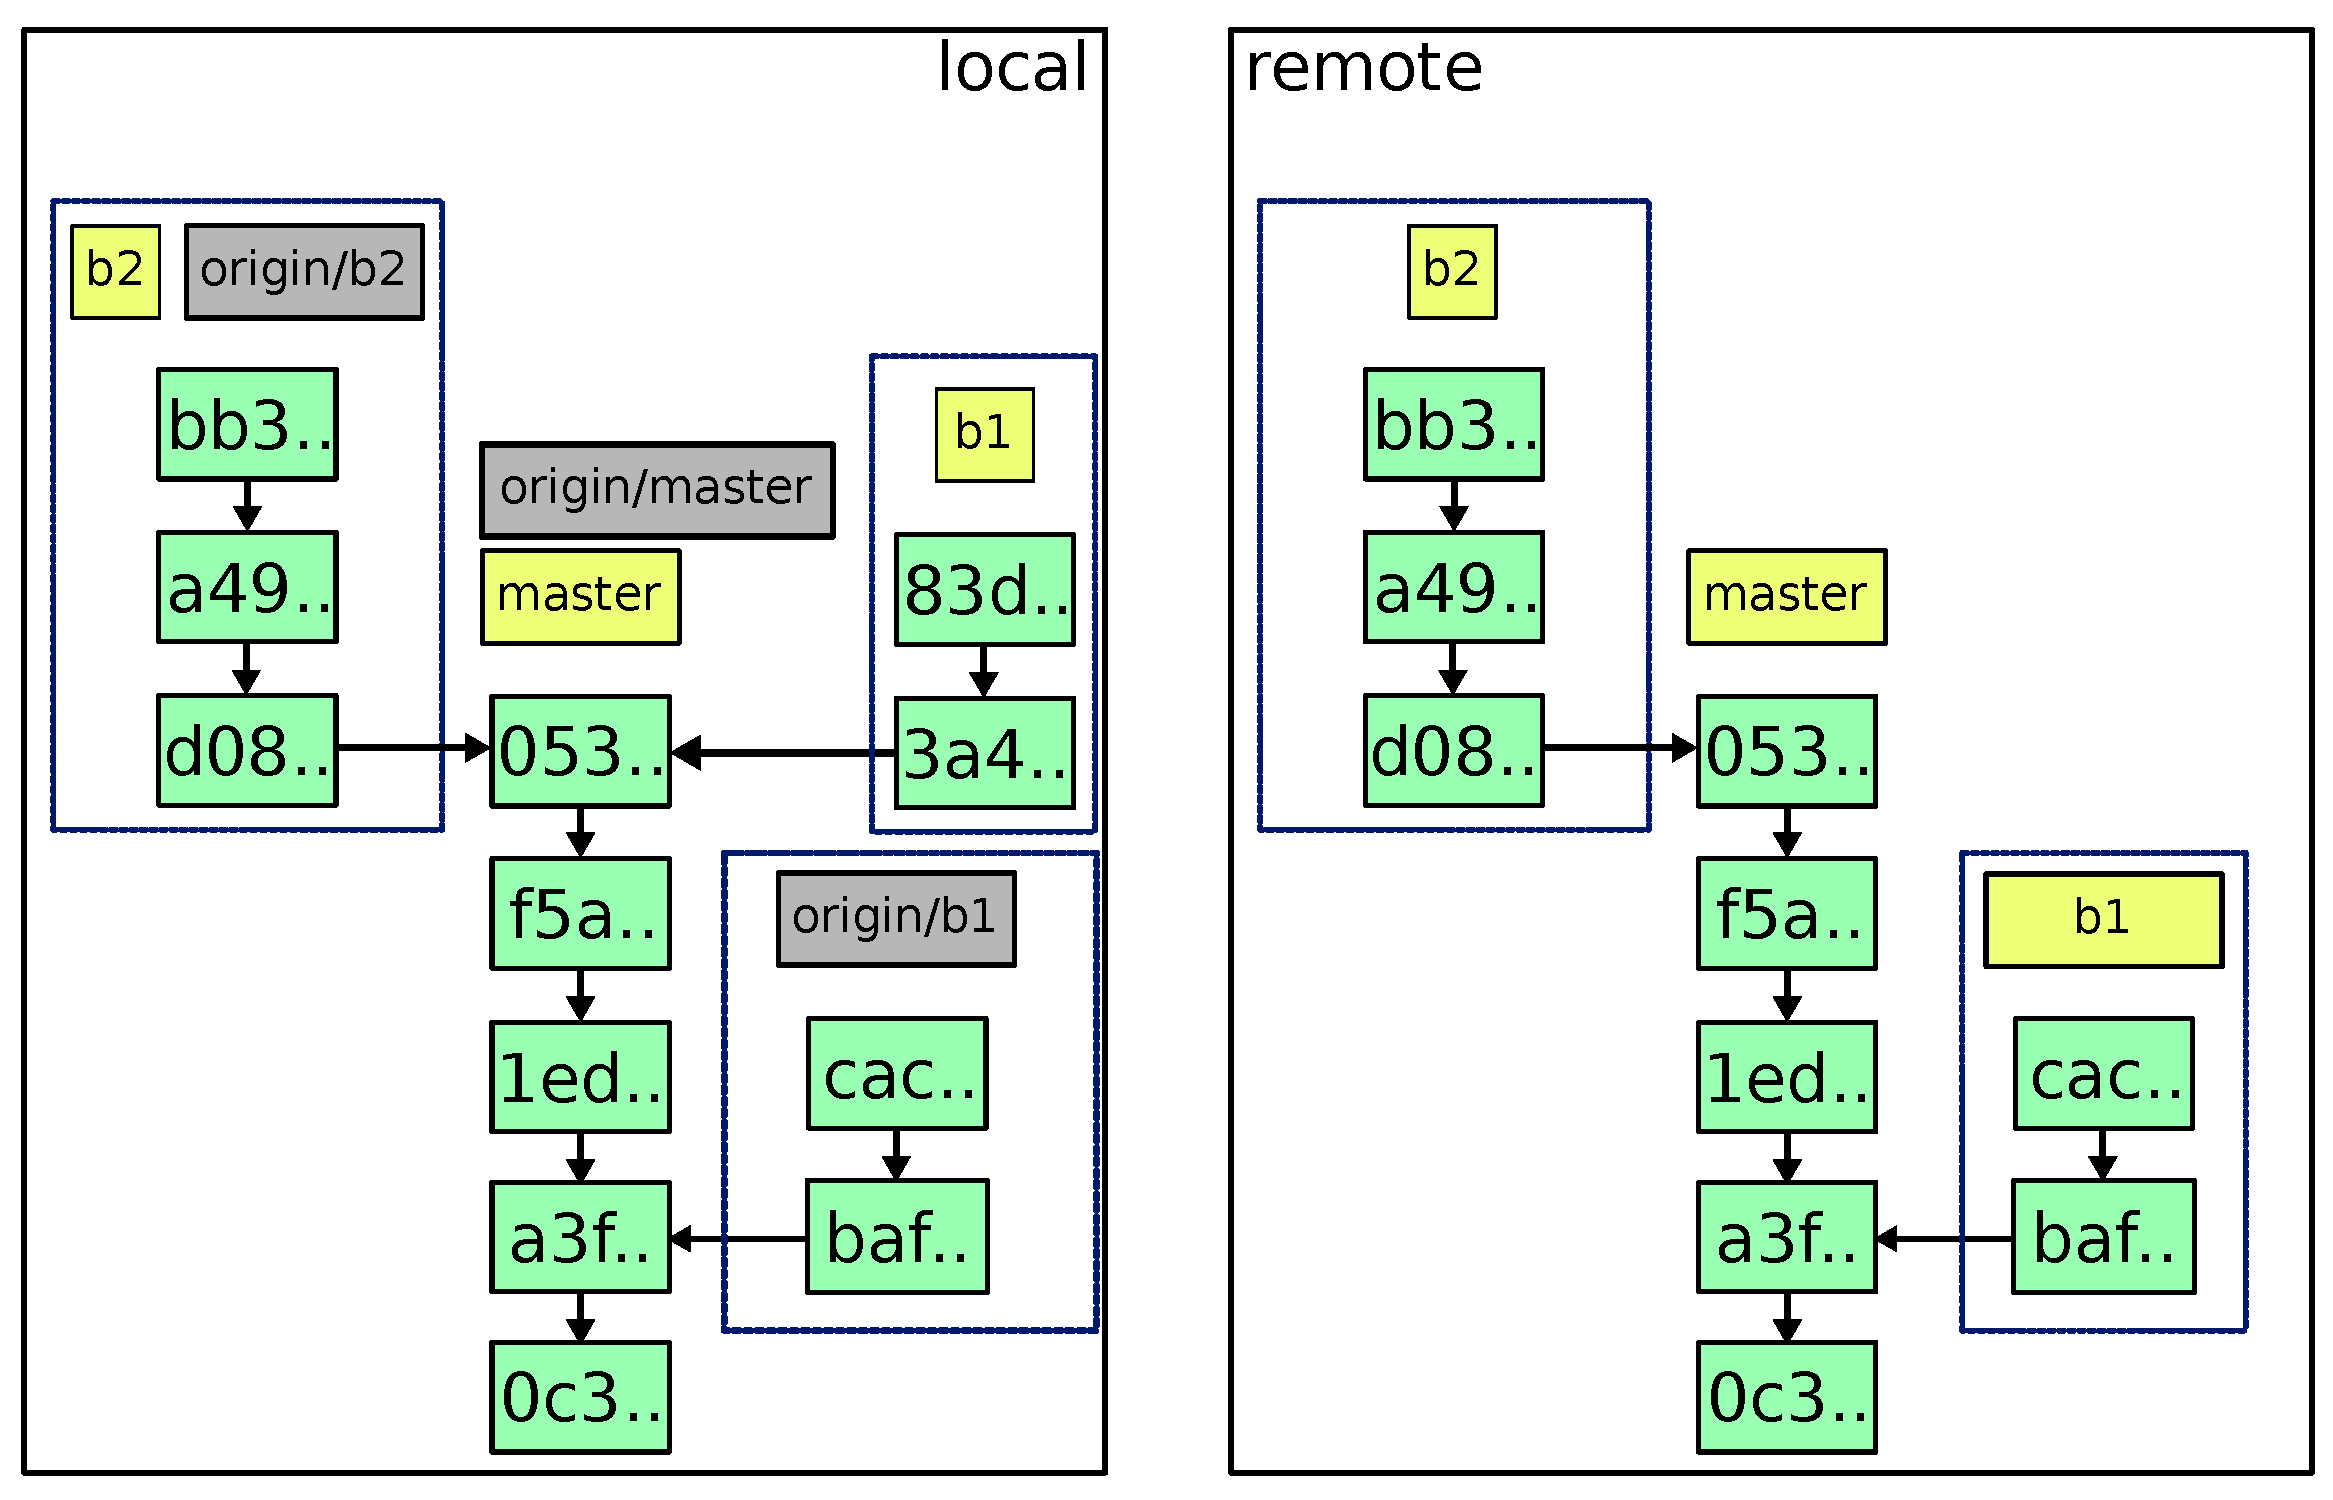
\includegraphics[width=\textwidth]{img/5.pdf}
\end{frame}

\begin{frame}{}
  \begin{itemize}
  \item \lstinline|git push -f origin b1|
  \end{itemize}
\end{frame}

\begin{frame}{}
  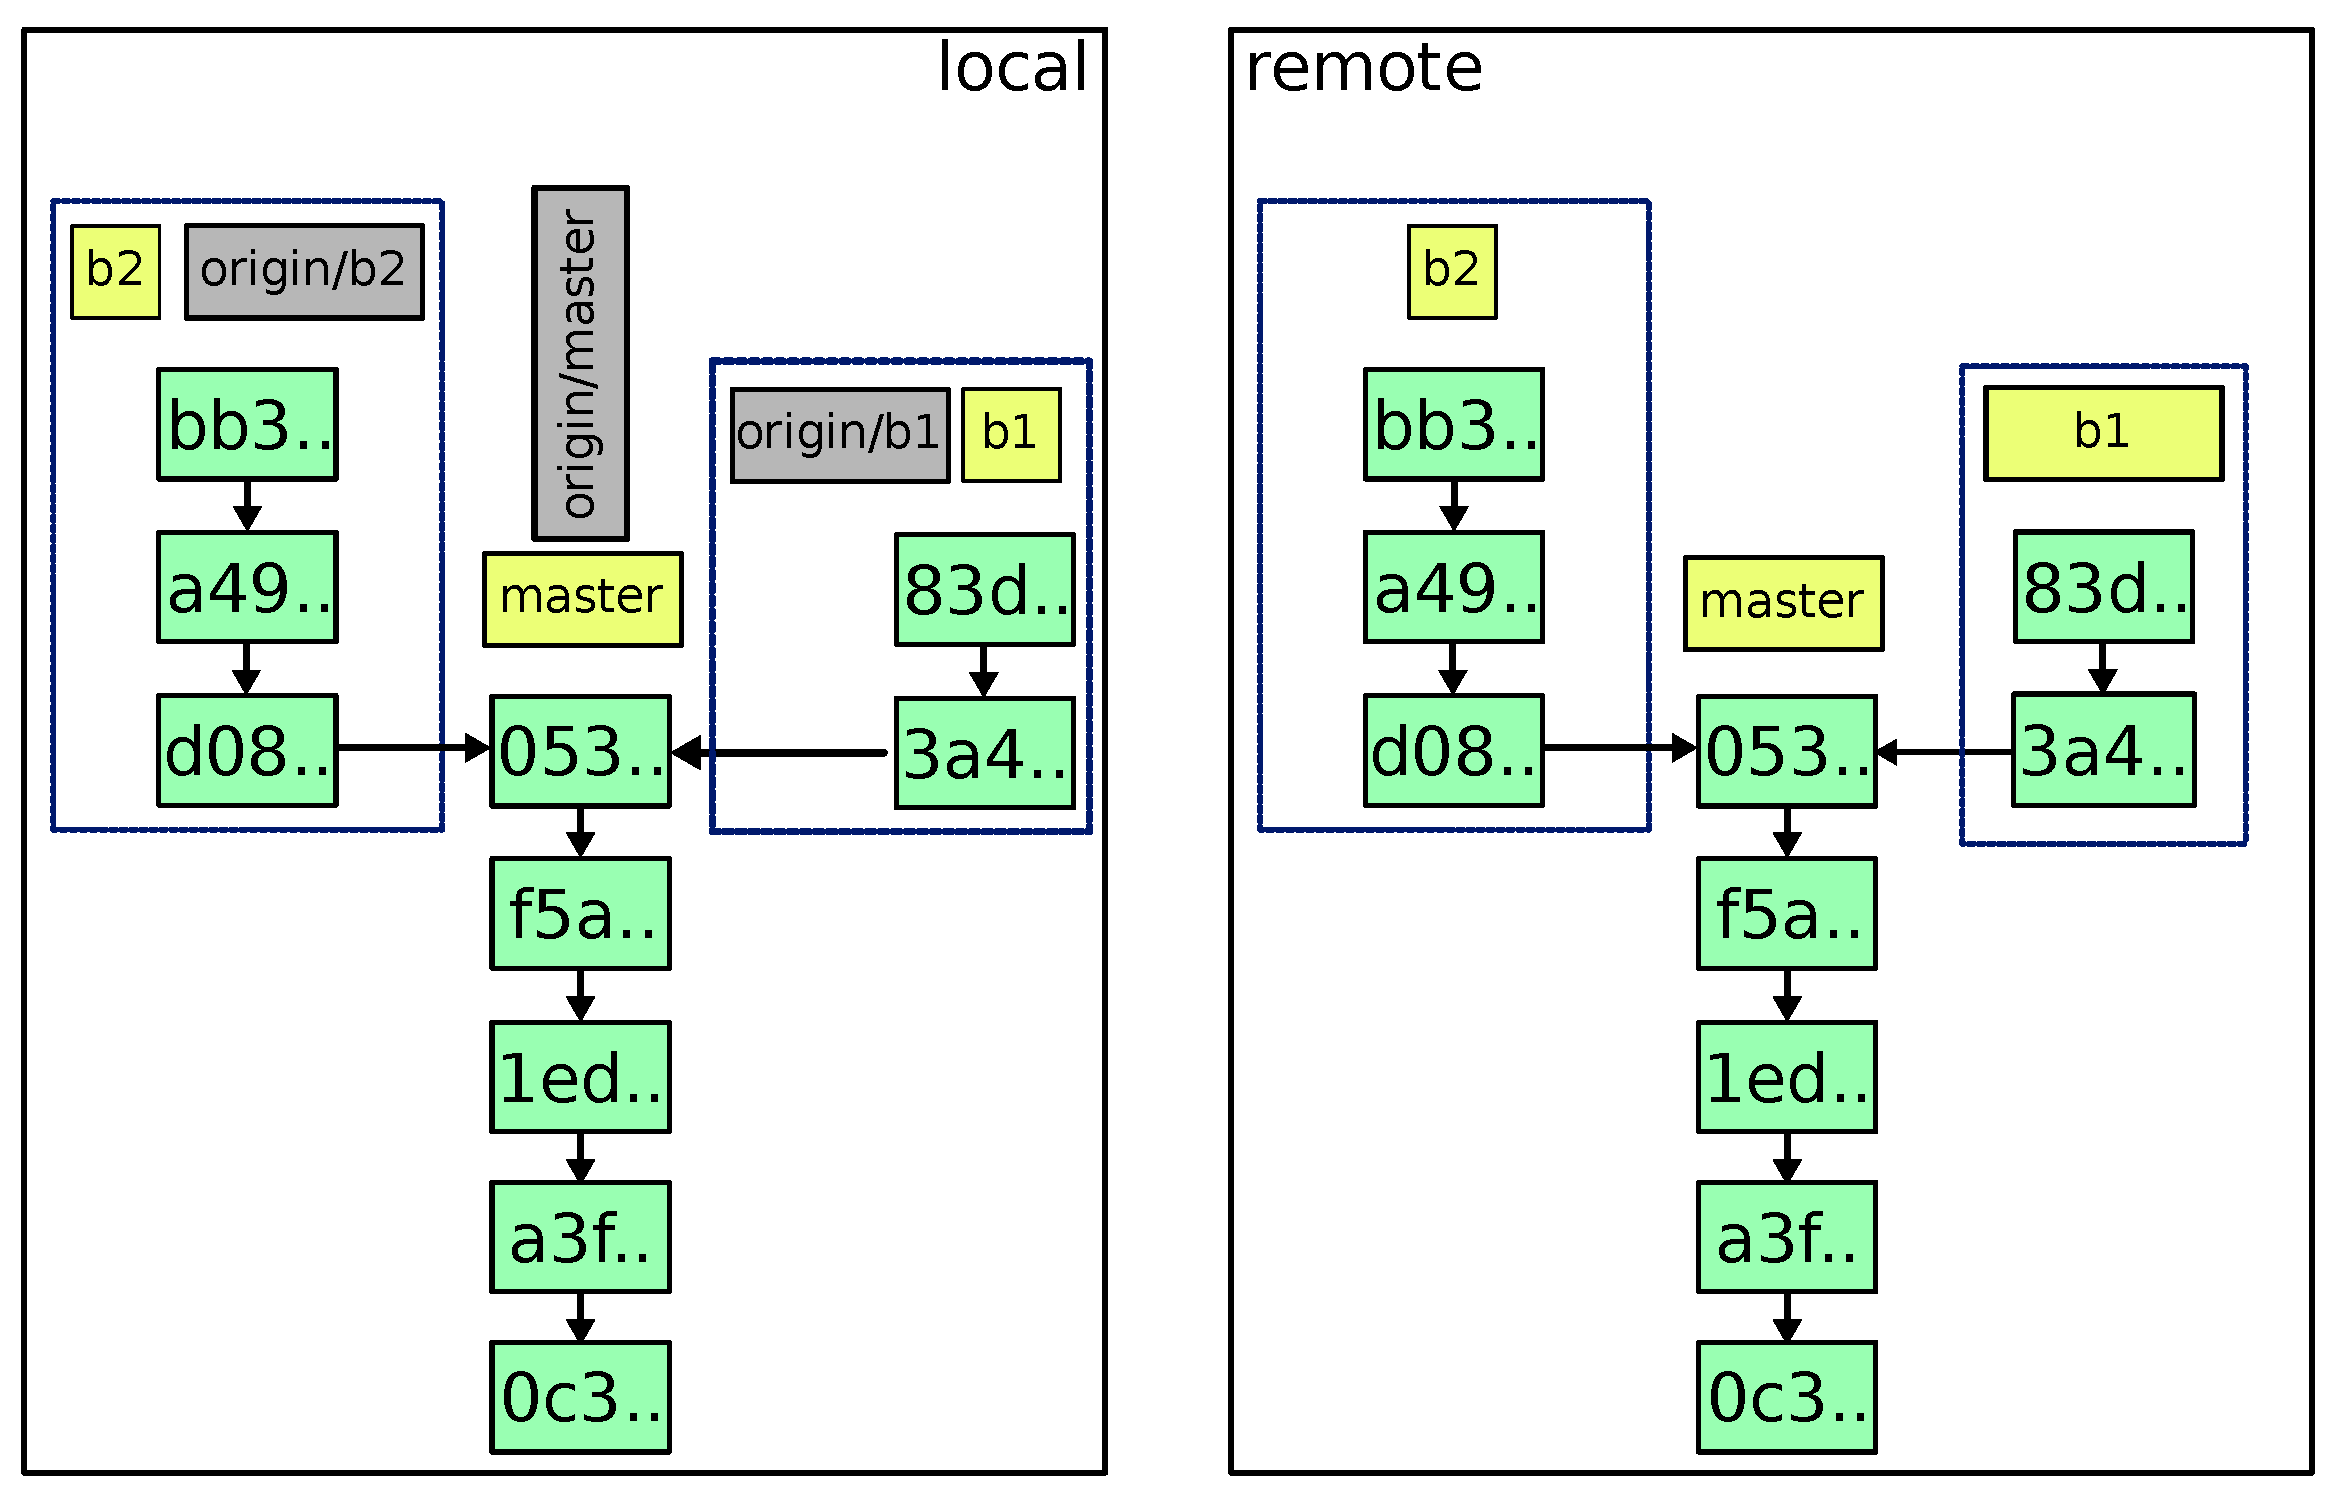
\includegraphics[width=\textwidth]{img/6.pdf}
\end{frame}

\begin{frame}{}
  \begin{itemize}
  \item \lstinline|git push origin b1:master|
  \end{itemize}
\end{frame}

\begin{frame}{}
  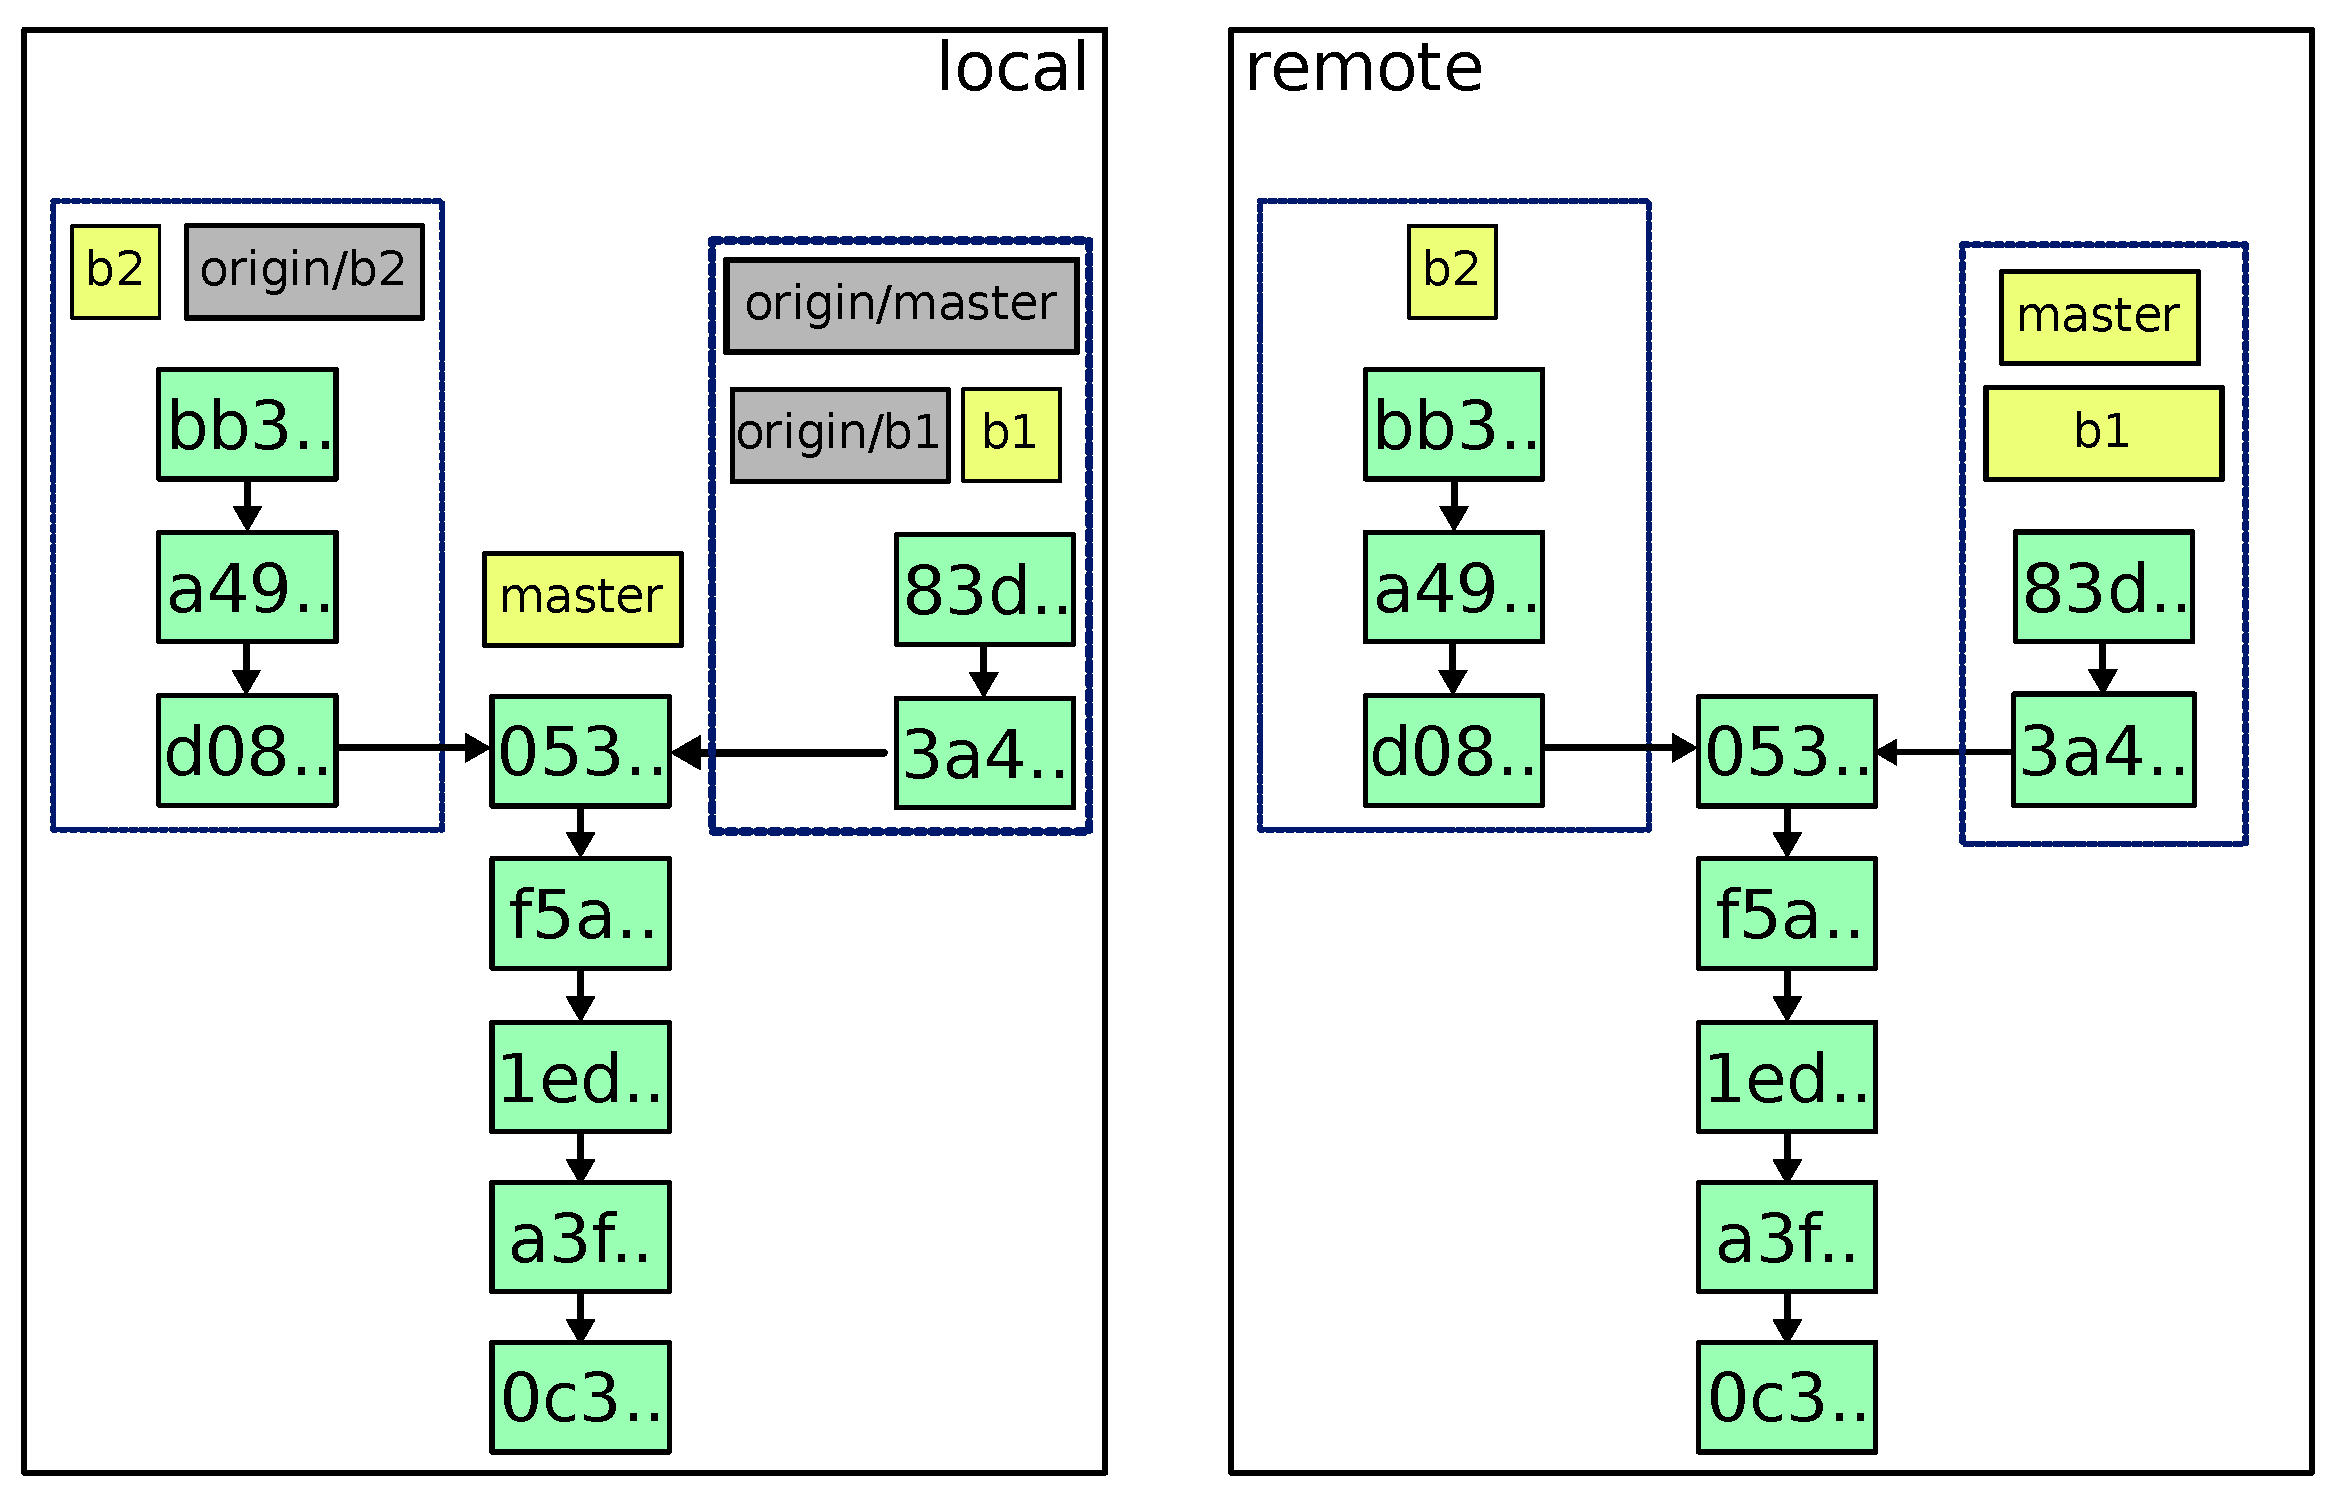
\includegraphics[width=\textwidth]{img/7.pdf}
\end{frame}

\begin{frame}{}
  \begin{itemize}
  \item \lstinline|git pull origin master|
  \item \lstinline|git branch -D b2|
  \item \lstinline|git push origin :b2|
  \end{itemize}
\end{frame}

\begin{frame}{}
  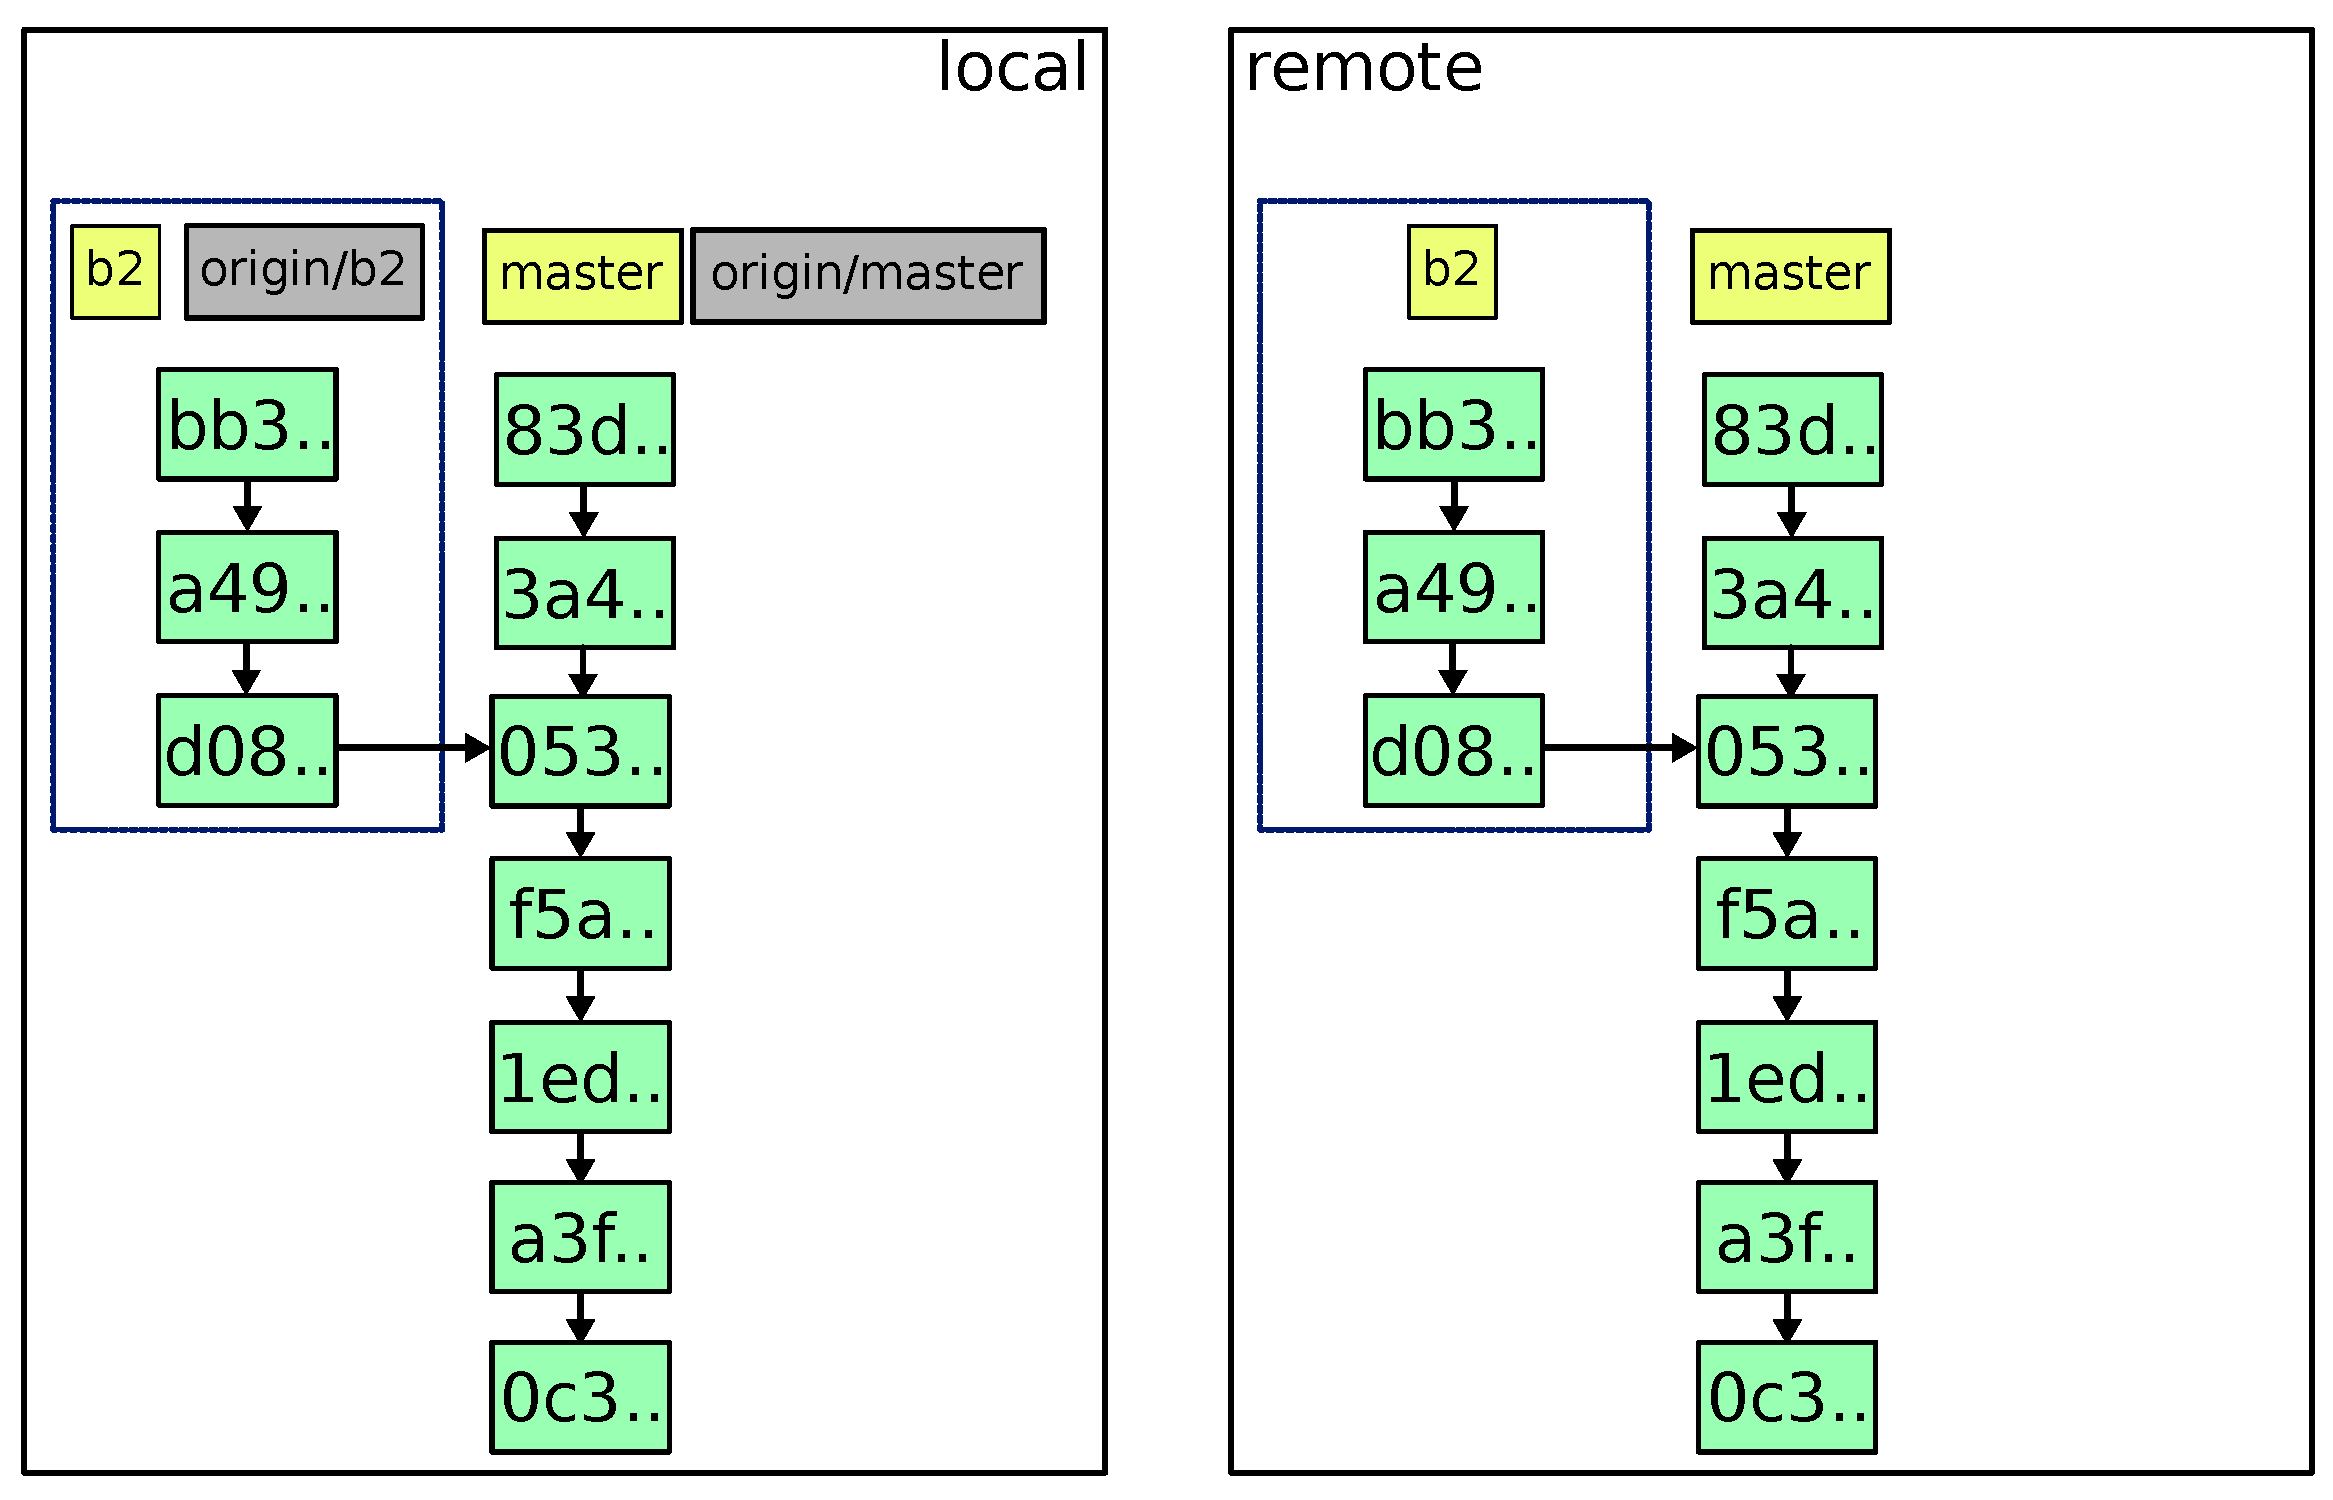
\includegraphics[width=\textwidth]{img/8.pdf}
\end{frame}

\begin{frame}{}
  \begin{itemize}
  \item \lstinline|git rebase master b2|
  \item \lstinline|git push origin b2|
  \end{itemize}
\end{frame}

\begin{frame}{}
  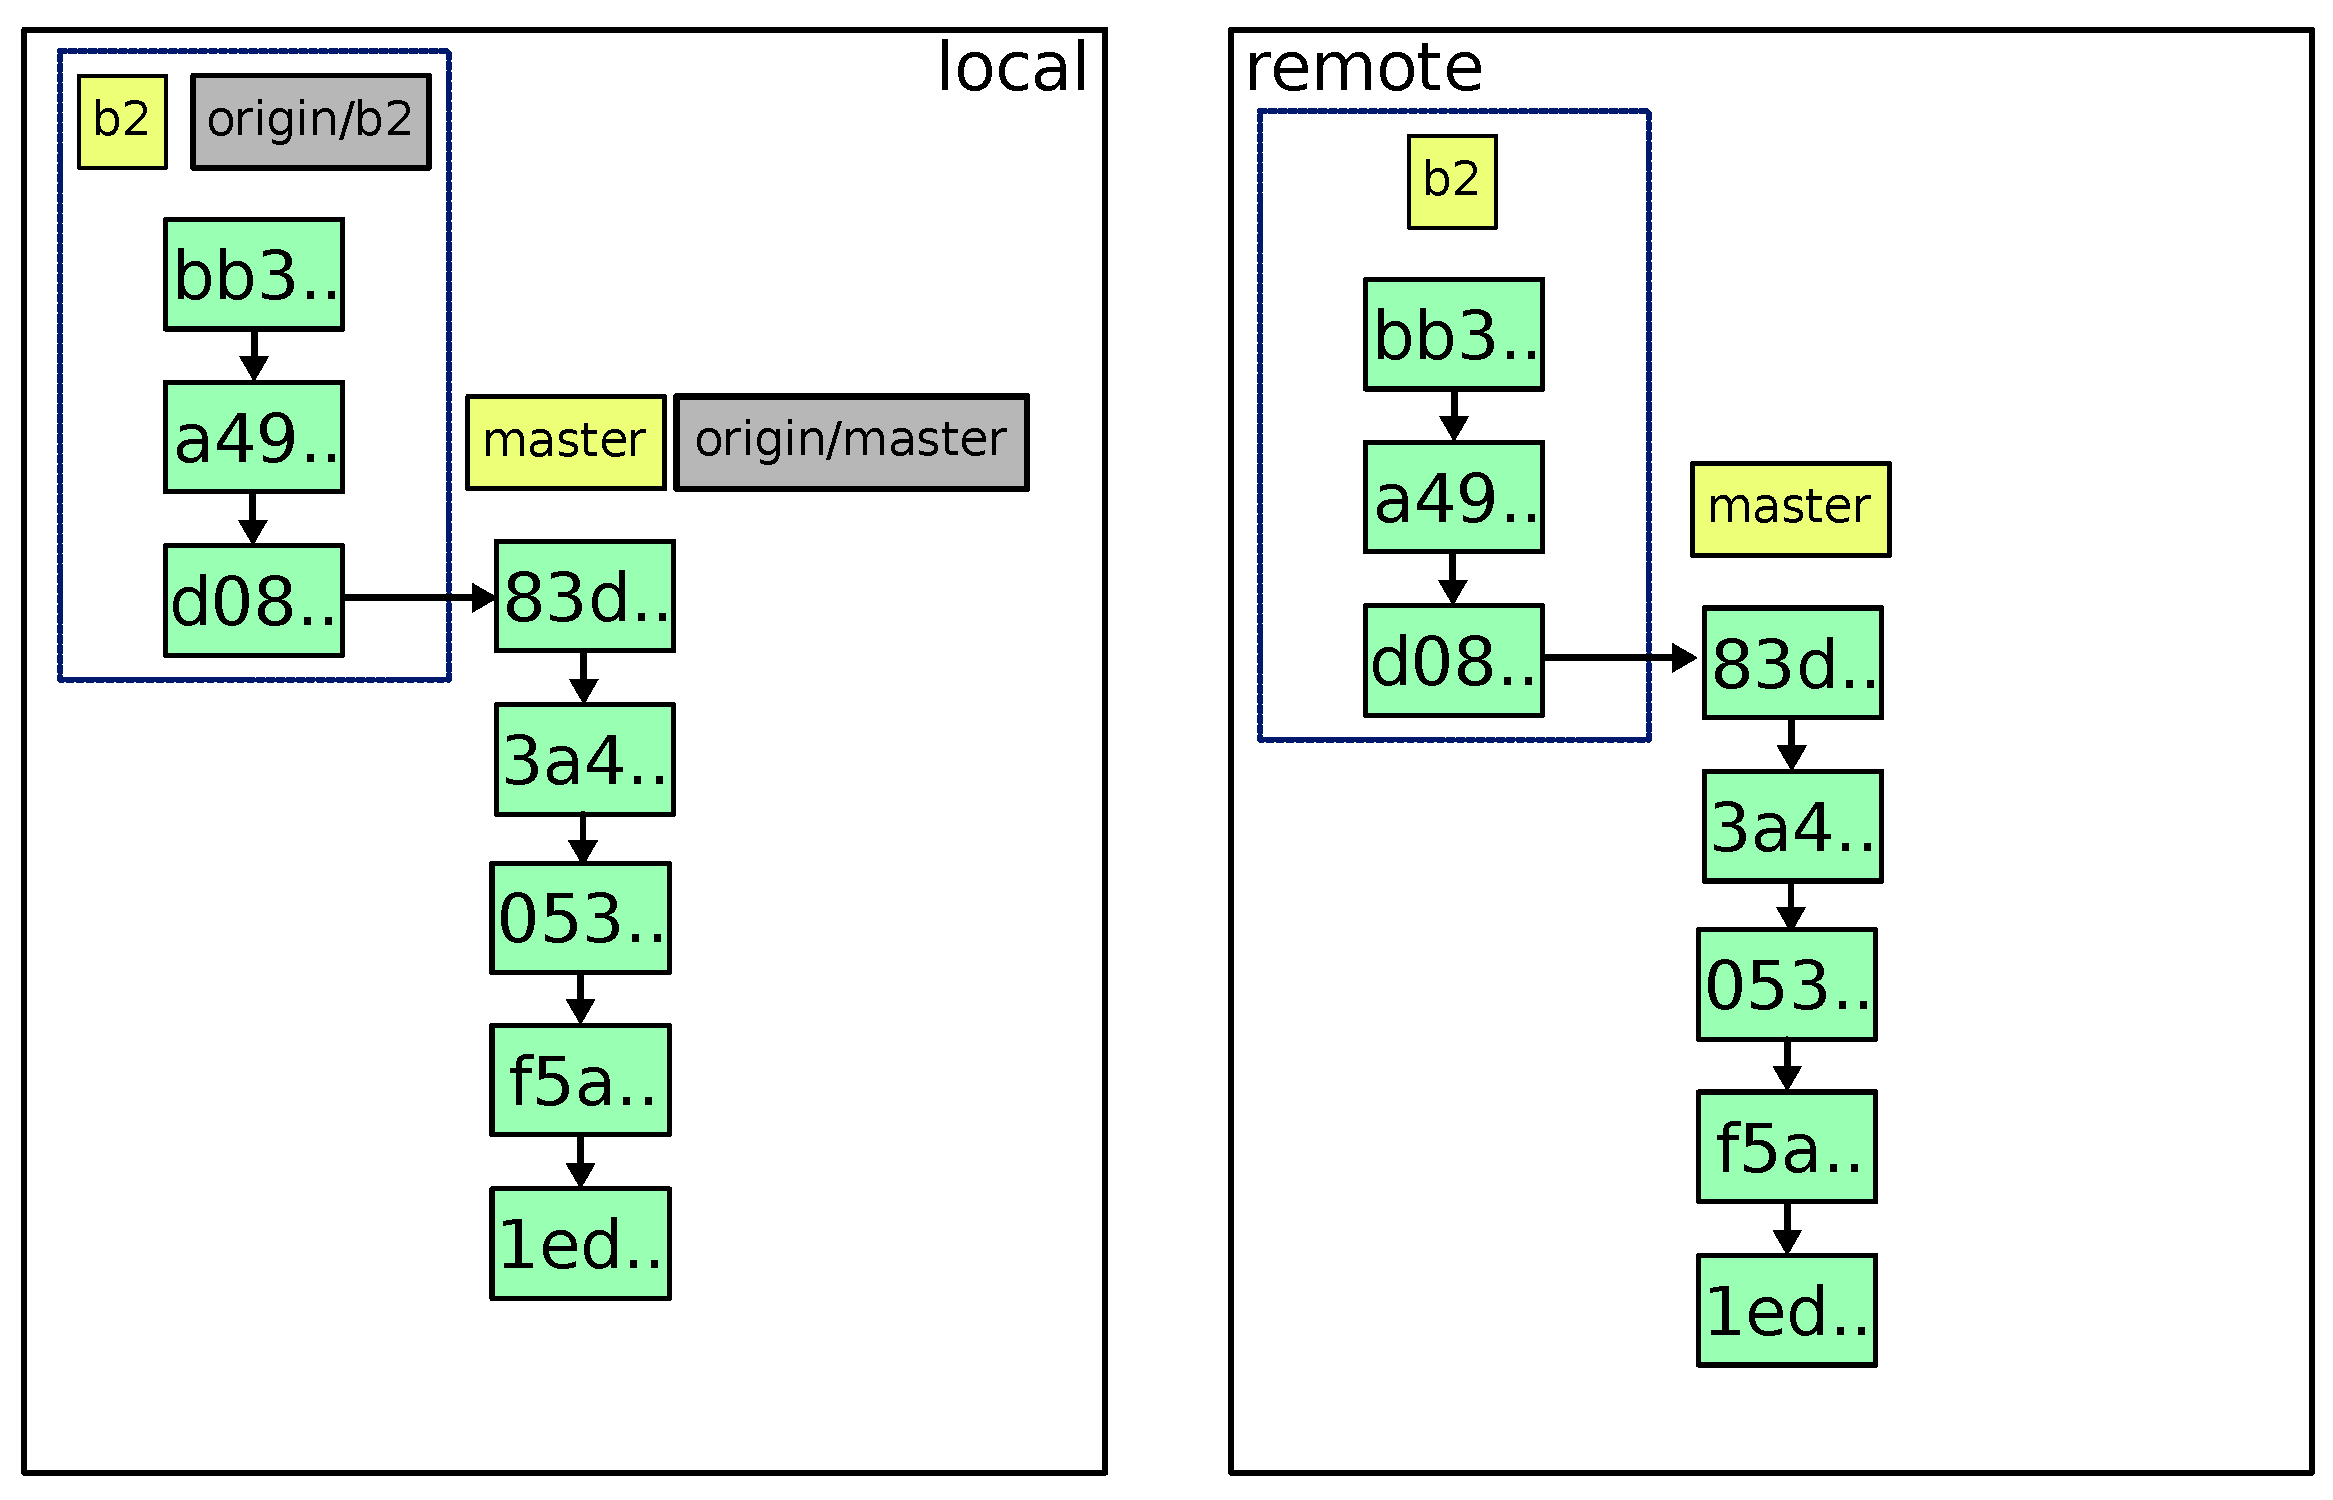
\includegraphics[width=\textwidth]{img/9.pdf}
\end{frame}

\begin{frame}{}
  \begin{itemize}
  \item \lstinline|git push origin b2:master|
  \item \lstinline|git branch -D b2|
  \item \lstinline|git push origin :b2|
  \item \lstinline|git pull origin master|
  \end{itemize}
\end{frame}

\begin{frame}{}
  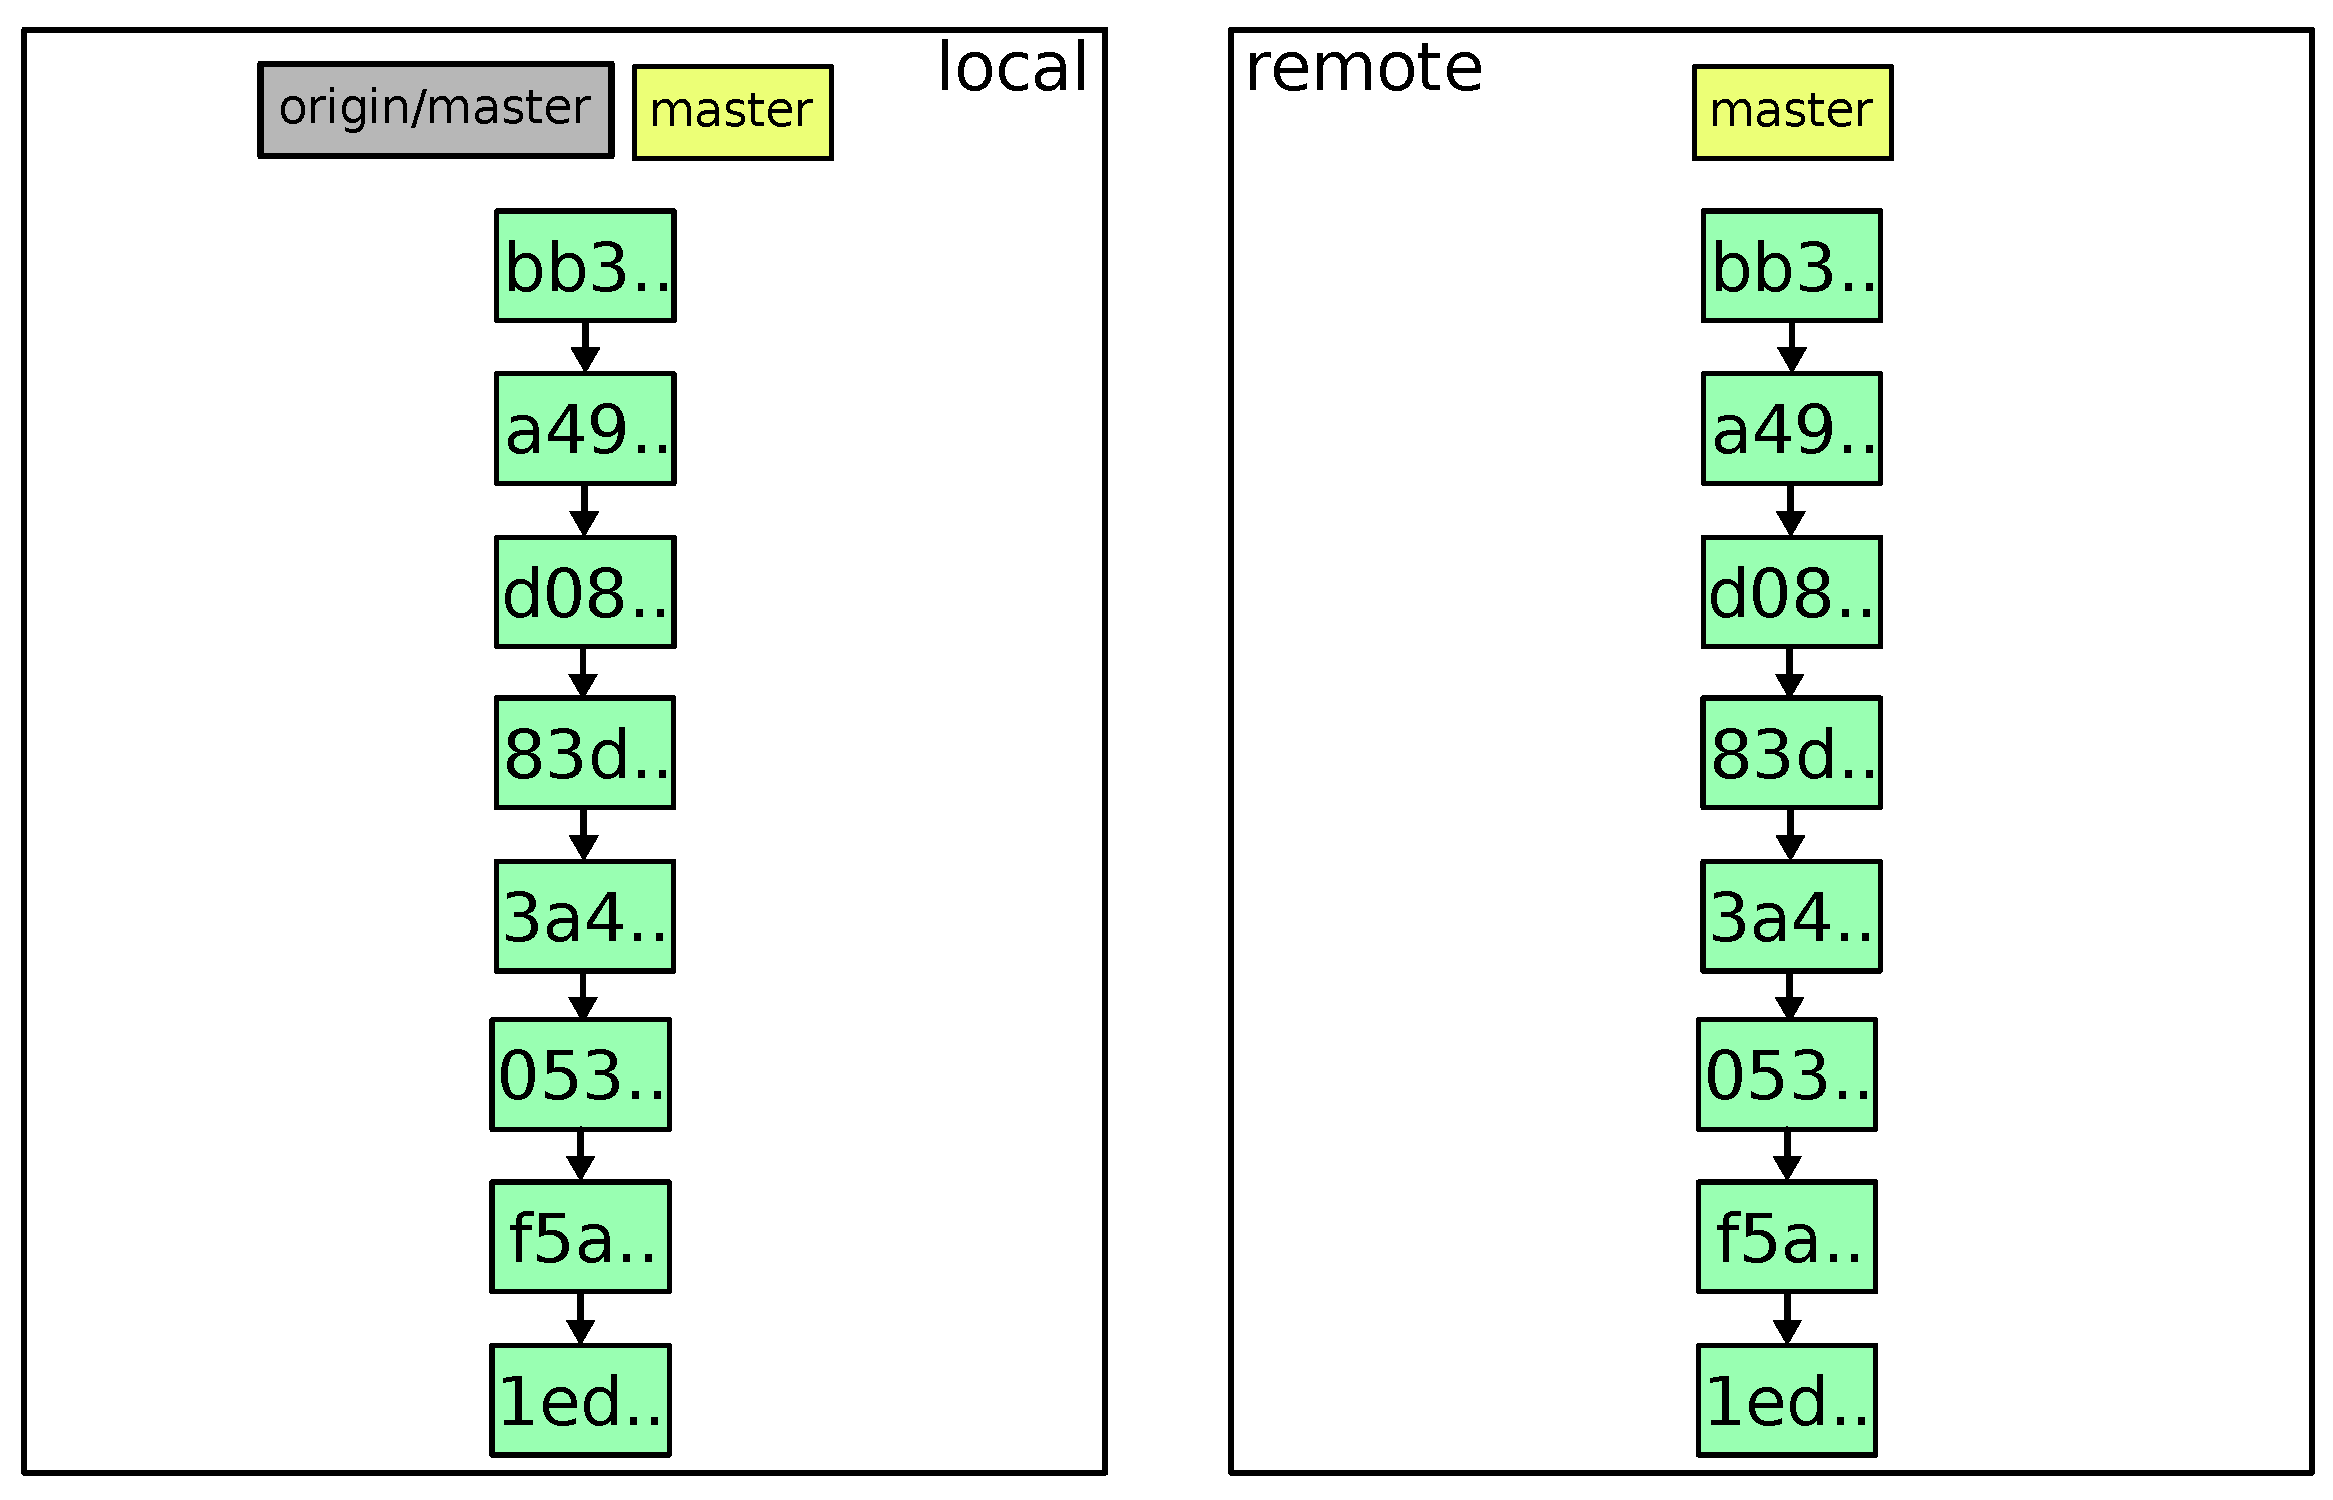
\includegraphics[width=\textwidth]{img/10.pdf}
\end{frame}

\begin{frame}{}
  \begin{center}
  \Huge \dots
  \end{center}
\end{frame}

%------------------------------------------------------------

\section{Ressources}
\begin{frame}{Ressources}
  \begin{itemize}
  \item \href{http://progit.org/about.html}{Progit}
  \item \href{http://git.or.cz/gitwiki/GitHosting}{Liste de serveurs \git}
  \end{itemize}
\end{frame}

\end{document}
